% -*- Mode:TeX -*-

%% IMPORTANT: The official thesis specifications are available at:
%%            http://libraries.mit.edu/archives/thesis-specs/
%%
%%            Please verify your thesis' formatting and copyright
%%            assignment before submission.  If you notice any
%%            discrepancies between these templates and the 
%%            MIT Libraries' specs, please let us know
%%            by e-mailing thesis@mit.edu

%% The documentclass options along with the pagestyle can be used to generate
%% a technical report, a draft copy, or a regular thesis.  You may need to
%% re-specify the pagestyle after you \include  cover.tex.  For more
%% information, see the first few lines of mitthesis.cls. 

%\documentclass[12pt,vi,twoside]{mitthesis}
%%
%%  If you want your thesis copyright to you instead of MIT, use the
%%  ``vi'' option, as above.
%%
%\documentclass[12pt,twoside,leftblank]{mitthesis}
%%
%% If you want blank pages before new chapters to be labelled ``This
%% Page Intentionally Left Blank'', use the ``leftblank'' option, as
%% above. 

\documentclass[12pt,twoside]{mitthesis}
\usepackage{lgrind}
%% These have been added at the request of the MIT Libraries, because
%% some PDF conversions mess up the ligatures.  -LB, 1/22/2014
\usepackage{cmap}
\usepackage{setspace}
\usepackage[T1]{fontenc}
\usepackage{mathtools}
\usepackage{graphicx}
\usepackage{epstopdf}
\usepackage{wrapfig}
\usepackage{caption}
\graphicspath{ {figures/} }
\pagestyle{plain}

\DeclareCaptionFormat{myformat}{#1#2#3\hrulefill}
\captionsetup[figure]{format=myformat}

%% This bit allows you to either specify only the files which you wish to
%% process, or `all' to process all files which you \include.
%% Krishna Sethuraman (1990).

\typein [\files]{Enter file names to process, (chap1,chap2 ...), or `all' to
process all files:}
\def\all{all}
\ifx\files\all \typeout{Including all files.} \else \typeout{Including only \files.} \includeonly{\files} \fi

\begin{document}
%\doublespace
\singlespace
% -*-latex-*-
% 
% For questions, comments, concerns or complaints:
% thesis@mit.edu
% 
%
% $Log: cover.tex,v $
% Revision 1.8  2008/05/13 15:02:15  jdreed
% Degree month is June, not May.  Added note about prevdegrees.
% Arthur Smith's title updated
%
% Revision 1.7  2001/02/08 18:53:16  boojum
% changed some \newpages to \cleardoublepages
%
% Revision 1.6  1999/10/21 14:49:31  boojum
% changed comment referring to documentstyle
%
% Revision 1.5  1999/10/21 14:39:04  boojum
% *** empty log message ***
%
% Revision 1.4  1997/04/18  17:54:10  othomas
% added page numbers on abstract and cover, and made 1 abstract
% page the default rather than 2.  (anne hunter tells me this
% is the new institute standard.)
%
% Revision 1.4  1997/04/18  17:54:10  othomas
% added page numbers on abstract and cover, and made 1 abstract
% page the default rather than 2.  (anne hunter tells me this
% is the new institute standard.)
%
% Revision 1.3  93/05/17  17:06:29  starflt
% Added acknowledgements section (suggested by tompalka)
% 
% Revision 1.2  92/04/22  13:13:13  epeisach
% Fixes for 1991 course 6 requirements
% Phrase "and to grant others the right to do so" has been added to 
% permission clause
% Second copy of abstract is not counted as separate pages so numbering works
% out
% 
% Revision 1.1  92/04/22  13:08:20  epeisach

% NOTE:
% These templates make an effort to conform to the MIT Thesis specifications,
% however the specifications can change.  We recommend that you verify the
% layout of your title page with your thesis advisor and/or the MIT 
% Libraries before printing your final copy.
\title{RNA Macrostates: Theory and Tools}

\author{Michael Flynn}
% If you wish to list your previous degrees on the cover page, use the 
% previous degrees command:
%       \prevdegrees{A.A., Harvard University (1985)}
% You can use the \\ command to list multiple previous degrees
%       \prevdegrees{B.S., University of California (1978) \\
%                    S.M., Massachusetts Institute of Technology (1981)}
\department{Department of Electrical Engineering and Computer Science}

% If the thesis is for two degrees simultaneously, list them both
% separated by \and like this:
% \degree{Doctor of Philosophy \and Master of Science}
\degree{Bachelor of Science in Computer Science and Engineering}

% As of the 2007-08 academic year, valid degree months are September, 
% February, or June.  The default is June.
\degreemonth{June}
\degreeyear{1990}
\thesisdate{May 18, 1990}

%% By default, the thesis will be copyrighted to MIT.  If you need to copyright
%% the thesis to yourself, just specify the `vi' documentclass option.  If for
%% some reason you want to exactly specify the copyright notice text, you can
%% use the \copyrightnoticetext command.  
%\copyrightnoticetext{\copyright IBM, 1990.  Do not open till Xmas.}

% If there is more than one supervisor, use the \supervisor command
% once for each.
\supervisor{Daniel Aalberts}{Professor of Physics}

% This is the department committee chairman, not the thesis committee
% chairman.  You should replace this with your Department's Committee
% Chairman.
%\chairman{Arthur C. Smith}{Chairman, Department Committee on Graduate Theses}

% Make the titlepage based on the above information.  If you need
% something special and can't use the standard form, you can specify
% the exact text of the titlepage yourself.  Put it in a titlepage
% environment and leave blank lines where you want vertical space.
% The spaces will be adjusted to fill the entire page.  The dotted
% lines for the signatures are made with the \signature command.
\maketitle

% The abstractpage environment sets up everything on the page except
% the text itself.  The title and other header material are put at the
% top of the page, and the supervisors are listed at the bottom.  A
% new page is begun both before and after.  Of course, an abstract may
% be more than one page itself.  If you need more control over the
% format of the page, you can use the abstract environment, which puts
% the word "Abstract" at the beginning and single spaces its text.

%% You can either \input (*not* \include) your abstract file, or you can put
%% the text of the abstract directly between the \begin{abstractpage} and
%% \end{abstractpage} commands.

% First copy: start a new page, and save the page number.
\cleardoublepage
% Uncomment the next line if you do NOT want a page number on your
% abstract and acknowledgments pages.
% \pagestyle{empty}
\setcounter{savepage}{\thepage}
%\begin{abstractpage}
%% $Log: abstract.tex,v $
% Revision 1.1  93/05/14  14:56:25  starflt
% Initial revision
% 
% Revision 1.1  90/05/04  10:41:01  lwvanels
% Initial revision
% 
%
%% The text of your abstract and nothing else (other than comments) goes here.
%% It will be single-spaced and the rest of the text that is supposed to go on
%% the abstract page will be generated by the abstractpage environment.  This
%% file should be \input (not \include 'd) from cover.tex.
In this thesis, I designed and implemented a compiler which performs
optimizations that reduce the number of low-level floating point operations
necessary for a specific task; this involves the optimization of chains of
floating point operations as well as the implementation of a ``fixed'' point
data type that allows some floating point operations to simulated with integer
arithmetic.  The source language of the compiler is a subset of C, and the
destination language is assembly language for a micro-floating point CPU.  An
instruction-level simulator of the CPU was written to allow testing of the
code.  A series of test pieces of codes was compiled, both with and without
optimization, to determine how effective these optimizations were.

%\end{abstractpage}

% Additional copy: start a new page, and reset the page number.  This way,
% the second copy of the abstract is not counted as separate pages.
% Uncomment the next 6 lines if you need two copies of the abstract
% page.
% \setcounter{page}{\thesavepage}
% \begin{abstractpage}
% % $Log: abstract.tex,v $
% Revision 1.1  93/05/14  14:56:25  starflt
% Initial revision
% 
% Revision 1.1  90/05/04  10:41:01  lwvanels
% Initial revision
% 
%
%% The text of your abstract and nothing else (other than comments) goes here.
%% It will be single-spaced and the rest of the text that is supposed to go on
%% the abstract page will be generated by the abstractpage environment.  This
%% file should be \input (not \include 'd) from cover.tex.
In this thesis, I designed and implemented a compiler which performs
optimizations that reduce the number of low-level floating point operations
necessary for a specific task; this involves the optimization of chains of
floating point operations as well as the implementation of a ``fixed'' point
data type that allows some floating point operations to simulated with integer
arithmetic.  The source language of the compiler is a subset of C, and the
destination language is assembly language for a micro-floating point CPU.  An
instruction-level simulator of the CPU was written to allow testing of the
code.  A series of test pieces of codes was compiled, both with and without
optimization, to determine how effective these optimizations were.

% \end{abstractpage}



\section*{Acknowledgments}

This is the acknowledgements section.  
%%%%%%%%%%%%%%%%%%%%%%%%%%%%%%%%%%%%%%%%%%%%%%%%%%%%%%%%%%%%%%%%%%%%%%
% -*-latex-*-

% Some departments (e.g. 5) require an additional signature page.  See
% signature.tex for more information and uncomment the following line if
% applicable.
% % -*- Mode:TeX -*-
%
% Some departments (e.g. Chemistry) require an additional cover page
% with signatures of the thesis committee.  Please check with your
% thesis advisor or other appropriate person to determine if such a 
% page is required for your thesis.  
%
% If you choose not to use the "titlepage" environment, a \newpage
% commands, and several \vspace{\fill} commands may be necessary to
% achieve the required spacing.  The \signature command is defined in
% the "mitthesis" class
%
% The following sample appears courtesy of Ben Kaduk <kaduk@mit.edu> and
% was used in his June 2012 doctoral thesis in Chemistry. 

\begin{titlepage}
\begin{large}
This doctoral thesis has been examined by a Committee of the Department
of Chemistry as follows:

\signature{Professor Jianshu Cao}{Chairman, Thesis Committee \\
   Professor of Chemistry}

\signature{Professor Troy Van Voorhis}{Thesis Supervisor \\
   Associate Professor of Chemistry}

\signature{Professor Robert W. Field}{Member, Thesis Committee \\
   Haslam and Dewey Professor of Chemistry}
\end{large}
\end{titlepage}


\pagestyle{plain}
  % -*- Mode:TeX -*-
%% This file simply contains the commands that actually generate the table of
%% contents and lists of figures and tables.  You can omit any or all of
%% these files by simply taking out the appropriate command.  For more
%% information on these files, see appendix C.3.3 of the LaTeX manual. 
\tableofcontents
\newpage
\listoffigures
\newpage
\listoftables


%% This is an example first chapter.  You should put chapter/appendix that you
%% write into a separate file, and add a line \include{yourfilename} to
%% main.tex, where `yourfilename.tex' is the name of the chapter/appendix file.
%% You can process specific files by typing their names in at the 
%% \files=
%% prompt when you run the file main.tex through LaTeX.
\newcommand{\stack}[2]{\begin{array}{c}{ #1 \\ #2 }\end{array}}

\chapter{Introduction}

\section{RNA Secondary Structure Prediction}

In the nucleus of a cell, RNA is constantly being synthesized by
transcribing sections of DNA onto a portable chain of the nucleic
acids adenine, gaunine, cytozine, and uracil. These RNAs serve several
functions inside of the cell, including acting as:

\begin{description}
\item[mRNA:] `messanger RNA', which travel to ribosomes to serve as blueprints for
  proteins,
\item[tRNA:] `transfer RNA', which bond to and transport amino acids
  to the ribosome to be formed into proteins,
\item[rRNA:] `ribosomal RNA', which make up ribosomes,
\item[ncRNAs] `non-coding RNAs', which are not involved in the
  manufacturing of proteins, instead being used as tools of the cell
  for tasks including the regulation of gene expression.
\end{description} 

The last group, ncRNAs, comprises the majority of RNAs synthesized and
have mostly unknown functions. It is unlikely that they just float
around the cell uselessly, rather they are the tools the cell uses to
build and run itself. It is also widely believed that the function of
a strand of RNA is directly related to its structure. While DNA is
composed of 2 seperate strands woven together in a double helix, RNA
is most often found as a single strand that folds back onto
itself. There are considered to be 3 main levels of structure of
RNA. The first, the primary structure, is the sequence of nucleic
acids that make up the strand of RNA i.e. `GACCUUGGGGCCCC...'. The
second, the secondary structure, is how these bases fold back on each
other and form base pairs, most often of the Watson and Crick variety
(`G-C', `A-U', although sometimes 'G-U' is possible as well). The
third, the tertiary structure, is how the structure bends on a larger
scale as the stems and loops formed by the secondary structure
interact with each other.

Primary structure can be readily observed by modern sequencing
technology, however it is the secondary structure that determines the
shape of the molecule, which is the most important when considering
interactions with other biological molecules. The full specification
of a secondary structure includes a list of every pair that is made by
2 of the nucleic bases in the primary structure making a bond. Finding
the secondary structure of an RNA molecule is a different task than
finding the primary structure of RNA because there is no single
solution for one chemical chain. For an individual RNA molecule there
are many valid pairings, in fact for a sequence of length $n$ there
are $O(1.8^n)$ secondary structures \cite{hofacker1998combinatorics}. 

To find which of these structures the molecule is likely to assume in
nature, we turn to statistical mechanics. We approximate the RNA
molecule as an isolated system in contact with a thermal resevoir that
is the cell, with each secondary structure as a state of that
system. In such a system the probability of any state $s$ is its
boltzmann factor divided by the partition function:

\begin{equation}
P(s) = \frac{1}{Z} e^{-\beta E(s)},
\end{equation}

where $\beta = \frac{1}{RT}$, $R$ is the gas constant, $T$ is the
temperature, and

\begin{equation}
Z = \sum_{s} e^{-\beta E(s)}.
\end{equation}

Initially researchers were satisfied with presenting the MFE (minimum
free energy) state as the state the molecule assumes in nature, after
all this state is the most probable. However it has become clear that
this analysis is unsufficient, as MFE structures still are not very
probable. Statistical procedures, sampling the Boltzmann distribution,
are a more modern tool for predicting the secondary structure found in
nature. 

\section{The Energy Model of RNA}

Computing the partition function and probabilities is impossible
without an energy model for RNA, $E(s)$. Setting the energy of the
single-stranded (no pair) state as $E = 0$, the energy model must
accurately estimate an energy for a folded secondary structure. In
chemical experiments, this can be measured by using a strand with an
known secondary structure and finding it's $\Delta G$ by deducing it
from the relative concentrations of single-stranded states to
double-stranded states in solution (see UV melting section).

%% historical notes and such
 The first energy models developed by researchers awarded energy
 bonuses to pairs formed. One of the first papers by Nussinov and
 Jacobson \cite{nussinov1980fast} awarded the same amount of points to
 A-U and G-C pairs and found the MFE state, so the algorithm reduced
 to finding the legal folding with the most base pairs. After, it was
 discovered exprimentally that G-C pairs are more stable than A-U
 pairs. Because of this, in further iterations the energy would be
 determined by counting hydrogen bonds of cannonically paired bases,
 assigning each -1 kcal/mol of free energy. This would mean that GC
 pairs are given -3 kcals/mol, AU and GU pairs are both given -2. The
 algorithm developed for this model minimized the free energy. Both
 this algorithm and the previous one had elementary dynamic
 programming solutions. They were useful models to use as a baseline,
 however, even the second iteration was not very accurate, on average
 only 20.5\% of known base pairs are correctly predicted. Later energy
 models would use it as a control for the hypothesis that they
 increased secondary structure prediction accuracy
 \cite{mathews1999expanded}.

Indeed, much improvement was made over the hydrogen bond model by
expanding it to include what is now called the Nearest Neighbor
model. Experiments made it clear that energy of an RNA folding is not
just linearly dependent on the bonds that are made. There are
significant interaction effects between nearby bases and bonds, this
is called `sequence dependence', and there are polymer physics based
energy terms that scale logarithmically with the length of a loop
(this can be thought of as the energy it takes to bend the strand). To
handle these interaction effects in a model, we approximate that they
are contained within loop regions. We divide our structure into its
loops and compute the energy of each loop, with a seperate energy
model for each.

\begin{figure}[t]
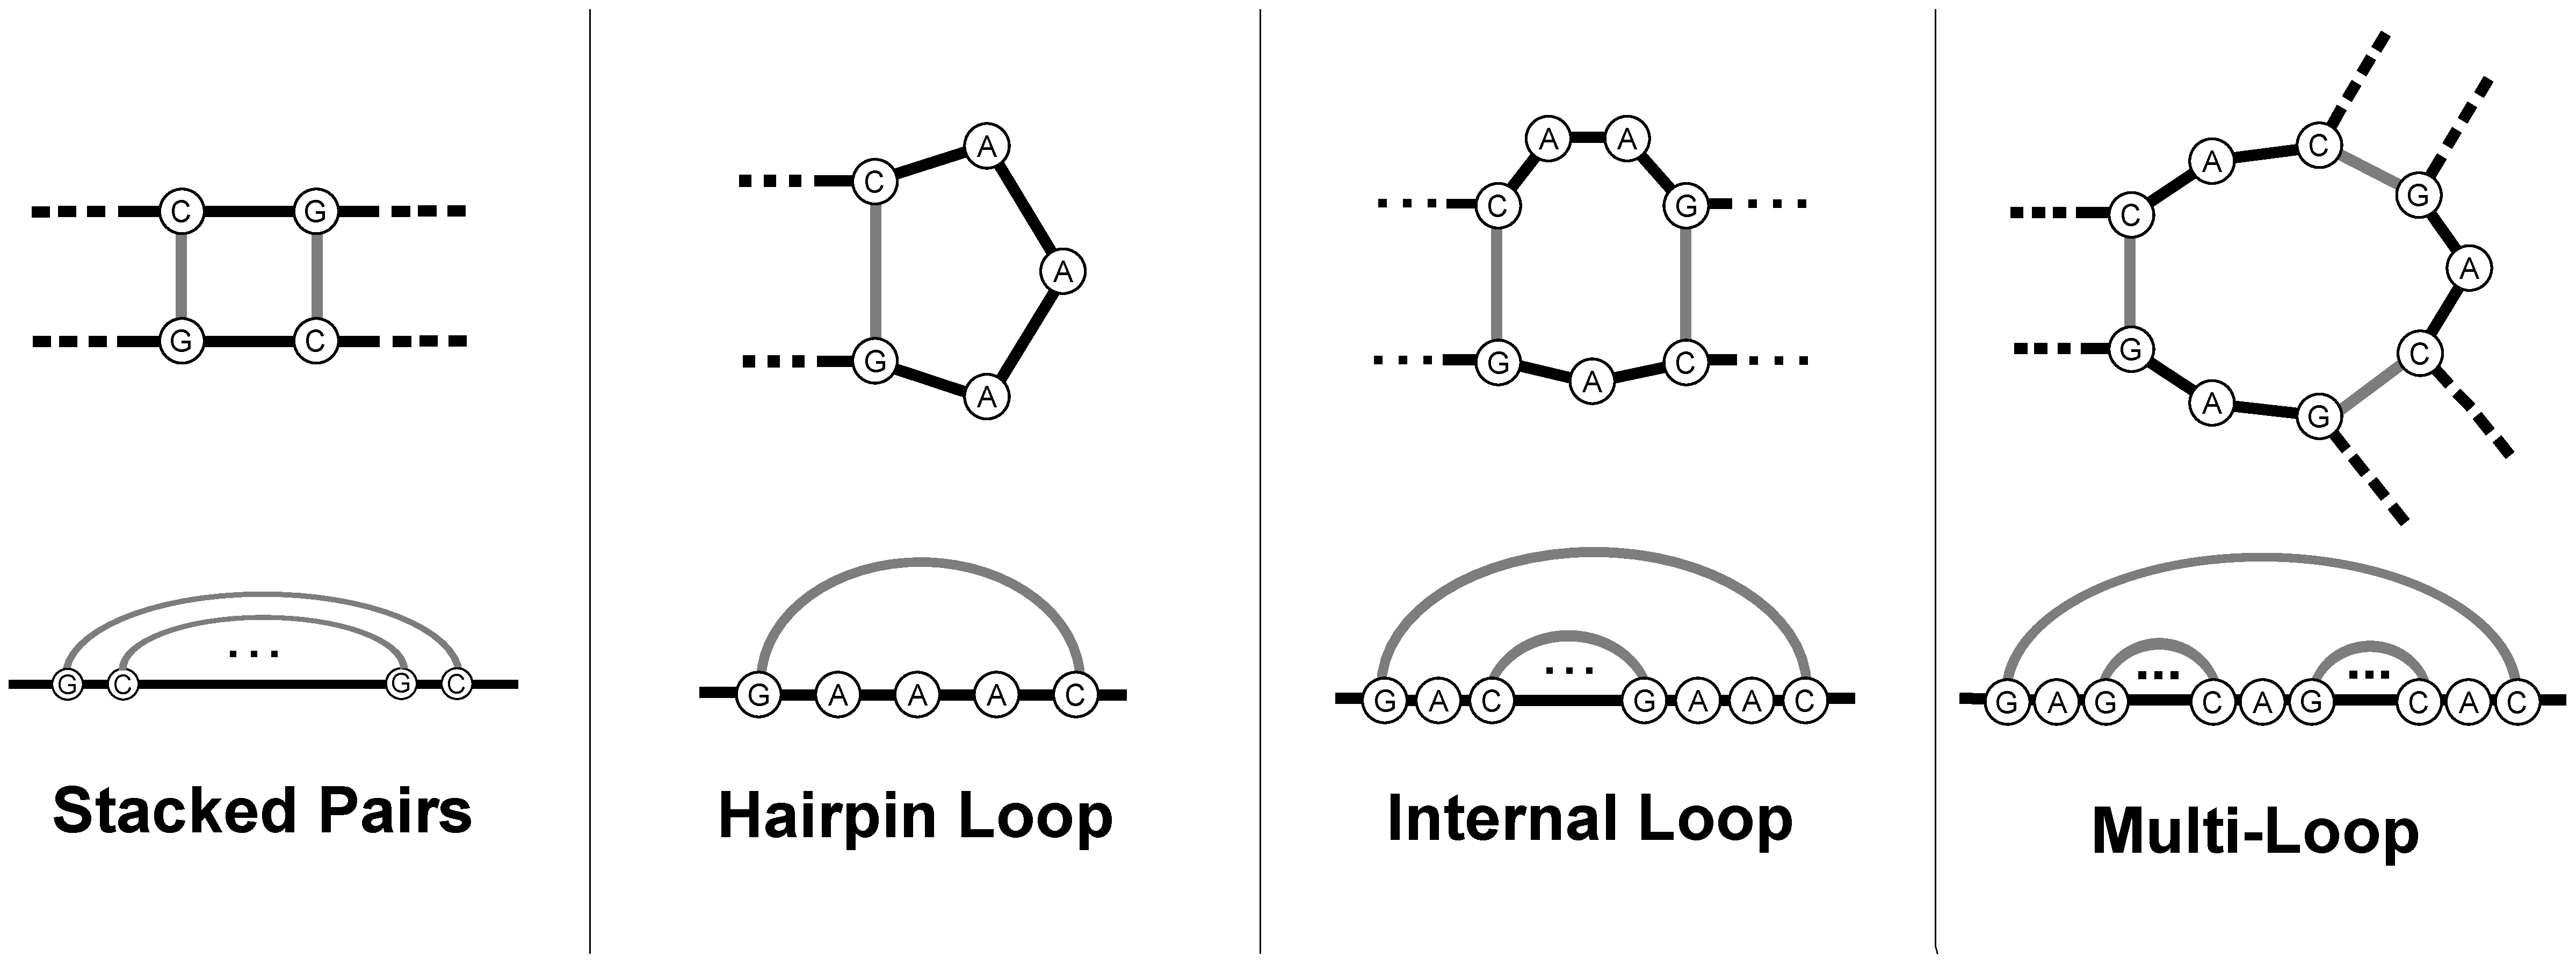
\includegraphics[width=\textwidth]{full_loop_figure.eps}
\caption{The 4 types of loops, black connections are bonds in the RNA
  backbone, grey connections are hydrogen bonds between bases. The
  types are: \textit{Stacked Pairs}, adjacent pairs of bonded bases,
  \textit{Hairpin Loops}, one bonding pair closing off a turn in the
  RNA backbone, \textit{Internal Loops}, which can range from bulges
  to long loops, connecting to pairs with 2 chains of unpaired bases,
  and \textit{Multi-Loops}, which  connect 3 or more pairs.}
\label{fig:loopFigure}
\end{figure}

In Figure \ref{fig:loopFigure}, these loops are described. In brief,
there is a different category and energy model for each type of loop
with different numbers of paired and unpaired bases. For example a
stack loop has 2 pairs and no unpaired bases. An internal loop has 2
pairs and arbitrary unpaired bases. A hairpin has 1 pair and arbitrary
unpaired bases. Finally a multi-loop has at least 3 pairs and
arbitrary unpaired bases. 

There is a 5th type of loop, called a pseudoknot. A pseudoknot
consists of 2 ``crossing'' pairs. This breaks the standard topology of
the loop diagrams and makes computation of the partition function
provably NP-hard [TODO: cite]. For this reason, pseudoknots are
excluded from consideration. This is not ideal because pseudoknots do
appear in nature, notably in ribosomal RNA (Mathews et al
1999). However, some of the results of this reseach might make the
computation of a certain restricted set of pseduoknots much more
efficient. 

[TODO: pseudoknot figure]

\subsection{Loop Parameters} 

One might wonder what the parameters, the terms, of this model would
be. The model is simply that the energy of a structure, is the sum of it's loops:

\begin{equation}
E(s) = \sum_{l \in \text{loops}} E(l).
\end{equation}

For example for a very predictably folding strand 'GGGAAACCC' (G's
really want to pair with C's and A's resist pairing), we can decompose
the energy as such:

\begin{equation}
\Delta G \left ( \vcenter{\hbox{ 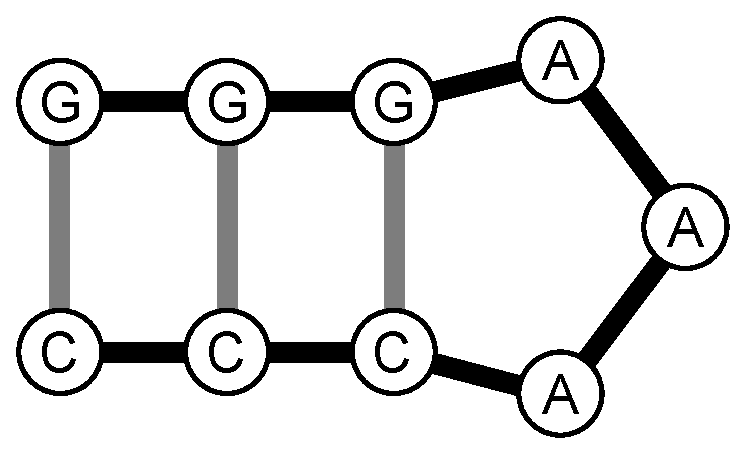
\includegraphics[scale=0.25]{stem_loop.eps}}}
 \right ) =
\Delta G_S \left ( \vcenter{\hbox{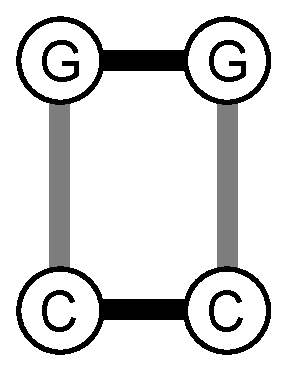
\includegraphics[scale=0.25]{GGCC-loop.eps}}}
\right ) +
\Delta G_S \left ( \vcenter{\hbox{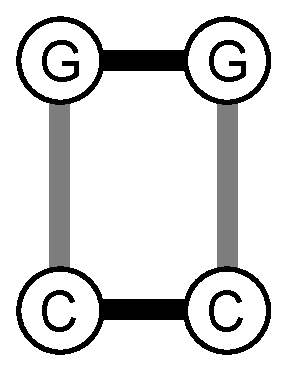
\includegraphics[scale=0.25]{GGCC-loop.eps}}}
\right ) + 
\Delta G_H \left (\vcenter{\hbox{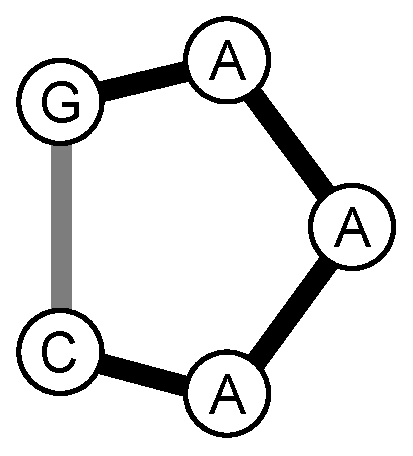
\includegraphics[scale=0.25]{stem_loop_hairpin.eps}}}
\right )
\label{eq:decomposition}
\end{equation}

Where $\Delta G_S$ is the function for energy of a stack loop and
$\Delta G_H$ is the function that gives you the energy of a hairpin
loop.

A model of loop energy should capture as much non-linearity as
possible. For stack loops, the legal pairings limit the possible loops
types. In fact, instead of worrying about how to model the loop's
energy using polymer physics, we can just exhaust the possible stack
loops, giving each a seperate parameter, i.e.

\begin{equation}
\Delta G_S \left ( \vcenter{\hbox{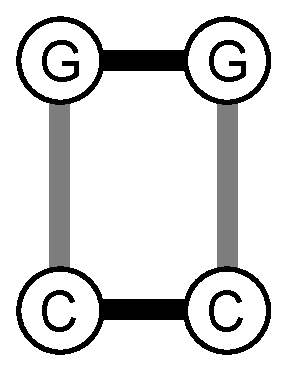
\includegraphics[scale=0.25]{GGCC-loop.eps}}}
\right ) = \beta_{S1}, \  
\Delta G_S \left ( \vcenter{\hbox{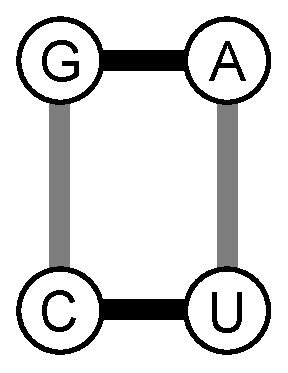
\includegraphics[scale=0.25]{GACU-loop.eps}}}
\right ) = \beta_{S2}, \ 
\Delta G_S \left ( \vcenter{\hbox{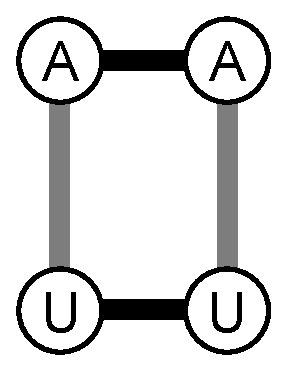
\includegraphics[scale=0.25]{AAUU-loop.eps}}}
\right ) = \beta_{S3}, \ \dots
\end{equation}

Where $\beta_{S1},\  \beta_{S2},\  \dots,\  \beta_{Sn}$ are parameters to a linear
regression model we fit to $\Delta G$ of `GGGAAACCC' and similar
sequences (see section: UV Melting Experiments). This is what is done in practice.

For the other type of loops, the sizes can grow unbounded, so simply
having a term for each loop will not work. However, at least for
internal and hairpin loops, in keeping with the nearest-neighbor
philosophy, we can keep a term for every combination of the bases that
start the loop, and then have a general term for computing the length,
addressing these both directly we have:

\paragraph{Hairpin Loop} 
Loops with 3 and 4 unpaired bases are kept in special tables of
triloop and tetraloop parameters, respectively. Each possible
tetraloop and triloop has it's own energy determined by
experiment. Beyond that, the general model is 
\begin{align}
\Delta G_H(n > 3) = & \Delta G_{init}(n) + \Delta
G_{HStack} (\text{Initializing Stack}) \\
&+ \Delta G (\text{bonuses}).
\end{align}

As you can see there is an initialization term and a stack term that
are both fitted via linear regression. The bonus term is for various
special loops that have been experimentally found to be more
stable. It's outside the scope of this thesis to get into them, but
they are specified in the paper by Mathews et al \cite{mathews1999expanded}.

\paragraph{Internal Loop}
Much like stack loops, internal loops are given individual parameters
for $1 \times 1$, $1 \times 2$, $2 \times 2$, internal loops, where $n
\times m$ denotes one arm of the loop having $n$ unpaired bases and
the other having $m$. This results from extensive studies on the
$\Delta G$'s of these internal loops. For the rest of internal loops
there's a model of the form:

\begin{align}
 \Delta G_{int} ( n \times m ) = \Delta G_{init} (n + m) + \Delta G_{asymmetry} (| n - m |) \\
& + \Delta G ( \text{bonuses}).
\end{align}

Where each term on the right is a regression parameter and the bonus
term is similar to the hairpin bonus term for loops composed and ended
with certain special kinds of bases determined experimentally to be
more stable.

\paragraph{Multi-Loops}
Multi-Loops are harder to create experimental strands for and because
of this there are no individual parameters for multi loops. In fact,
for modeling mutli-loops we regress to a more simple linear model of the form:
\begin{equation}
\Delta G_{multi} = a_1 + b_1 n + c_1 h + \Delta G_{dangle}
\end{equation}

Where $a_1$ is a penalty for starting a mutl-loop, $n$ is the number
of unpaired bases in the loop, $b_1$ is an energy penalty per unpaired
base, $h$ is the number of pairs in the structure, $c_1$ is the energy
bonus per pair, and $\Delta G_{dangle}$ is a term similar to stack
loop terms which include the energy of the unit composed of a pair and
its 2 adjacent unpaired bases, if it has them.

[TODO: coaxial stacking?]

\subsection{UV Melting experiments}

\begin{figure}[h]
\centering
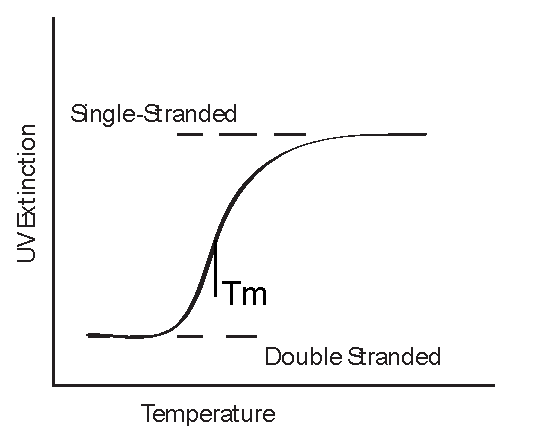
\includegraphics{MeltingGraph.eps}

\caption{An example of the output of a UV melting experiment. We
  should expect to see 2 levels of extinction in the graph, one
  corresopoding to where single-strandedness is the equilibrium
  condition of the strand and the other where double strandedness is
  the equilibrium. As the temperature increases, the strand absorbs
  more energy from the environment allowing it to escape the
  double-stranded state and so there is a transition interval where as
  the temperature increases the UV extinction goes from the
  double-stranded extinction to the single stranded extinction.[TODO:
    this graph has double stranded and single stranded extinction
    switched]}
\label{fig:UVMeltGraph}
\end{figure}

Loop regions are given energies as parameters to linear regression
models of free energy change in predictably folding strands. For
example, the strand `GGGAAACCC' folds predictably into a structure
with all the G's paired to the C's and a 3-A hairpin turn (because G's
pair very strongly to C's and A's tend to resist pairing) as seen in
Equation \ref{eq:decomposition}. Large amounts of identical strands
are synthesized and put into solution and heated. A two-state
assumption is made, either the RNA is folded in a `double-stranded'
state or unfolded in a `single-stranded' state. As the solution heats,
there is enough ambient energy to put all the strands in the unfolded,
no-bonds state. RNA is an organic, aromatic molecule that absobes
light in the UV spectrum in different amounts depending on whether it
is in a folded state or unfolded state, so the UV absobtion is fit to
a curve that then tells us about the relative concentrations of the
single-stranded vs. double-stranded state, which in turn tells us
about the free energy change between the two at a given
temperature. This free energy change is extracted and treated as a
function of the loop variables, which are then fitted to a linear
model over experiments on many different such strands
\cite{xia1998thermodynamic}.

For example, if we wanted to compute the free energy change of a
strand and fit it to it's loop parameters:

\begin{equation}
\Delta G \left ( \vcenter{\hbox{ 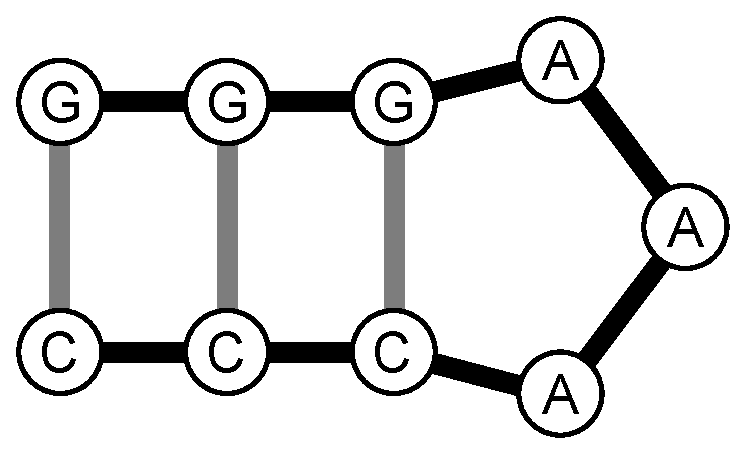
\includegraphics[scale=0.25]{stem_loop.eps}}}
 \right ) =
\Delta G_S \left ( \vcenter{\hbox{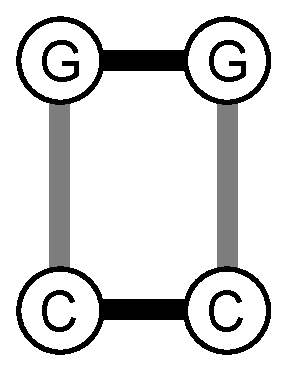
\includegraphics[scale=0.25]{GGCC-loop.eps}}}
\right ) +
\Delta G_S \left ( \vcenter{\hbox{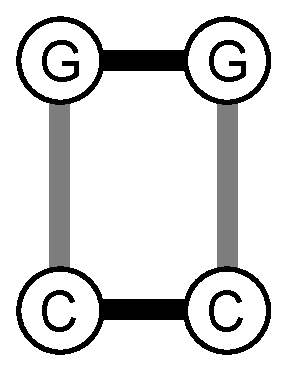
\includegraphics[scale=0.25]{GGCC-loop.eps}}}
\right ) + 
\Delta G_H \left (\vcenter{\hbox{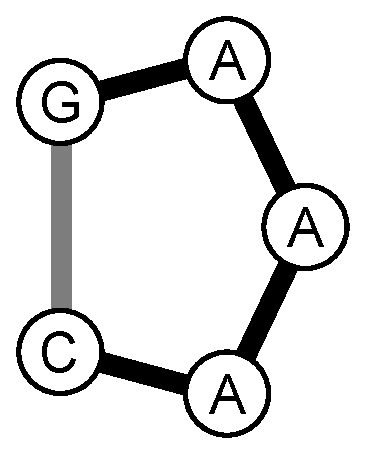
\includegraphics[scale=0.25]{GACA-hairpin.eps}}}
\right ) 
\end{equation}

We synthesize large amounts of the strand 'GGGAAACCC', put them in
solution and heat them and record their UV extinction. Observing the
curve to be like something in Figure \ref{fig:UVMeltGraph}. The
melting temperature $T_m$ is defined to be where the concentrations of
single stranded and double stranded molecules are equal, and this is
taken to be the inflection point of the graph in Figure
\ref{fig:UVMeltGraph}. From there Van't Hoof analysis is performed,
where the concentration, $C_T$, is varied and this follows a model of
the form:

\begin{equation}
  \frac{1}{T_m} = \frac{R}{\Delta H} \log{C_T} + \frac{\Delta S}{\Delta H}.
\end{equation}

This equation comes from the relation $\Delta G = -RT \log{K_{eq}}$
and plotting $1/T_m$ against $\log{C_T}$ and fitting a linear model
gives us the parameters $\Delta S$ and $\Delta H$ from the slope and
intercept and therefore $\Delta G$ through the relation

\begin{equation}
\Delta G = \Delta H - T \Delta S.
\end{equation}

If we repeat this process over several strands, we can then fit the
$\Delta G$'s to a linear model based on the many parameters described
in the Loop Parameters section. From there, when we want to compute
the energy of a folding, all we have to do is seperate it into loops
and sum the energies of each based off the parameters of this model.


%Without the use of cool graphics, we might notate the above as:
%
%\begin{equation}
%\Delta G (GGGAAACCC) = \Delta G_s \left ( \begin{array}{c} 3' C C 5 ' \\ 5' G G 3 ' \end{array} \right ) +
%\Delta G_S \left ( \begin{array}{c} 3' C C 5 ' \\ 5' G G 3 ' \end{array} \right ) +
%\Delta G_H (G AAA C)
%\end{equation}
%
%Where $\Delta G_S $ is an individual parameter for the stack loop
%energy term and $\Delta G_H$ contains the terms for the hairpin energy
%term.

\subsection{Example Energy Computation}

\begin{figure}[t]
  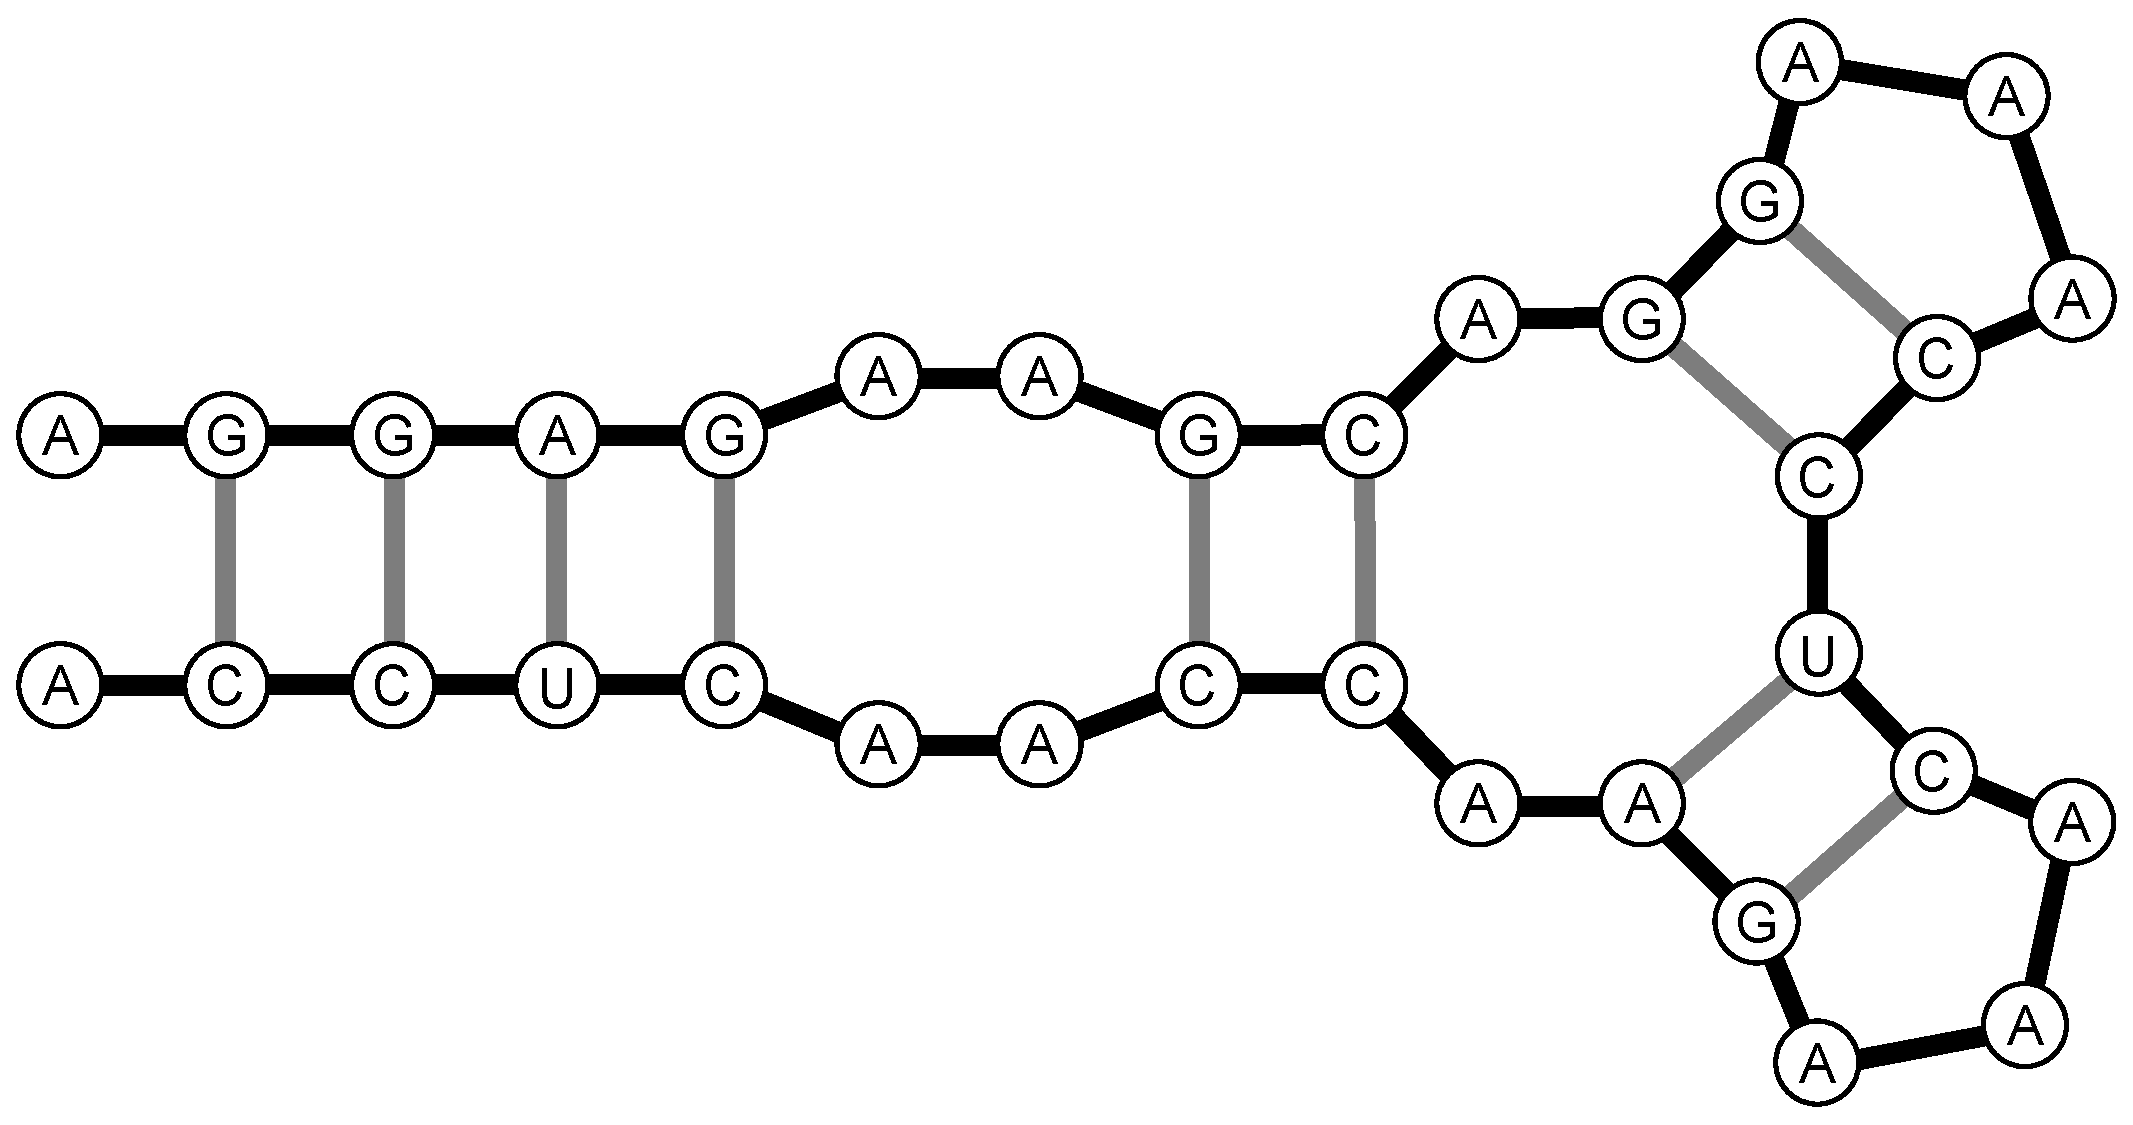
\includegraphics[width=\textwidth]{big_loop.eps}

  \captionsetup{singlelinecheck=off}
  \caption[.]{
    This is one possible folding out of the $O(1.8^n)$ secondary
    structures of the sequence
    `AGGAGAAGCAGGAAACCUCAAAGAACCAACUCCA'.    
  }
  \label{fig:bigLoop}
\end{figure}

Here's an example of the energy computation of a secondary structure,
pictured in Figure \ref{fig:bigLoop}. There are 3 stack loop of the type:
\begin{equation}
  \Delta G \left ( \vcenter{\hbox{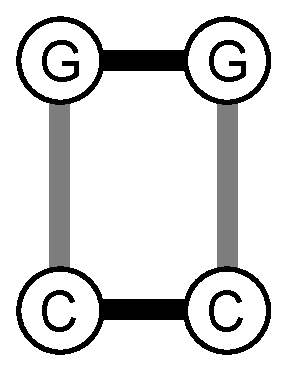
\includegraphics[scale=0.25]{GGCC-loop.eps}}}
  \right ) = -3.26 \text{ kcal/mol},
\end{equation}
and one of each:
\begin{align}
  &\Delta G \left ( \vcenter{\hbox{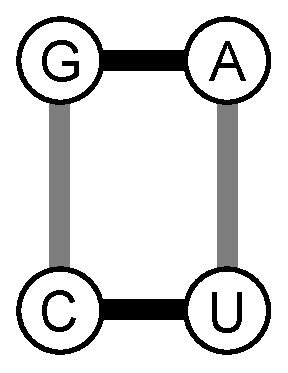
\includegraphics[scale=0.25]{GACU-loop.eps}}}
  \right ) = -2.35 \text{ kcal/mol},\\ 
  &\Delta G \left ( \vcenter{\hbox{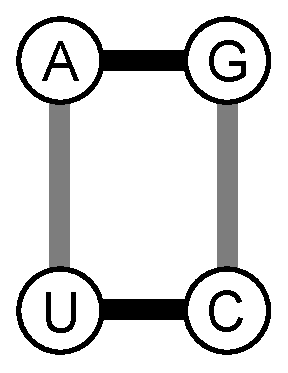
\includegraphics[scale=0.25]{AGUC-loop.eps}}}
  \right ) = -2.35 \text{ kcal/mol},\\
  &\Delta G \left ( \vcenter{\hbox{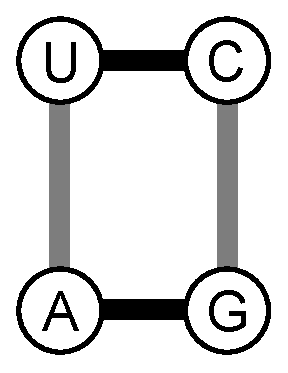
\includegraphics[scale=0.25]{UCAG-loop.eps}}}
  \right ) = -2.08 \text{ kcal/mol}.
\end{align}
These are all lookups from linear regression parameters. Besides the
stacks, there are 2 identical hairpins, an internal loop, an external
loop, and a multi-loop. For the hairpins the energy can be looked up
in a special parameter table designed specifically for hairpins with 3
unpaired bases called triloops:
\begin{align}
  \Delta G \left ( \vcenter{\hbox{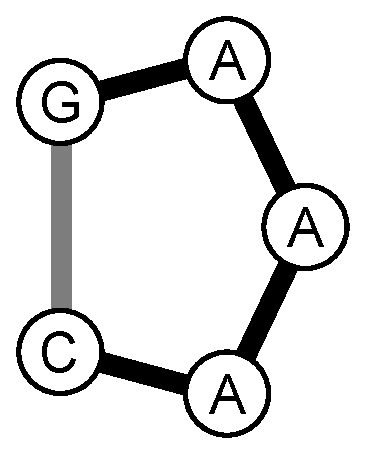
\includegraphics[scale=0.25]{GACA-hairpin.eps}}}
  \right ) &= 5.8
\end{align}

For the internal loop, there is a direct lookup for the $2 \times 2$
mismatch in a table:

\begin{align}
  \Delta G \left ( \vcenter{\hbox{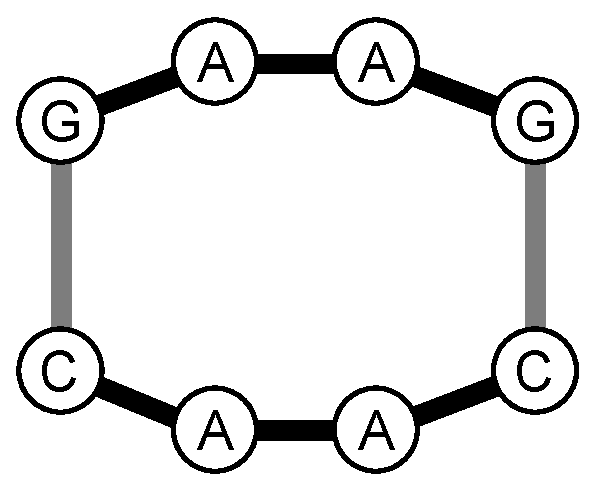
\includegraphics[scale=0.25]{GAAG-CAAC-internal-loop.eps}}}
  \right ) = 0.5 \text{ kcals/mol}.
\end{align}

The multibranch loop has 3 pairs and 2 unpaired bases. The energy is therefore:

\begin{align}
  \Delta G \left (\vcenter{\hbox{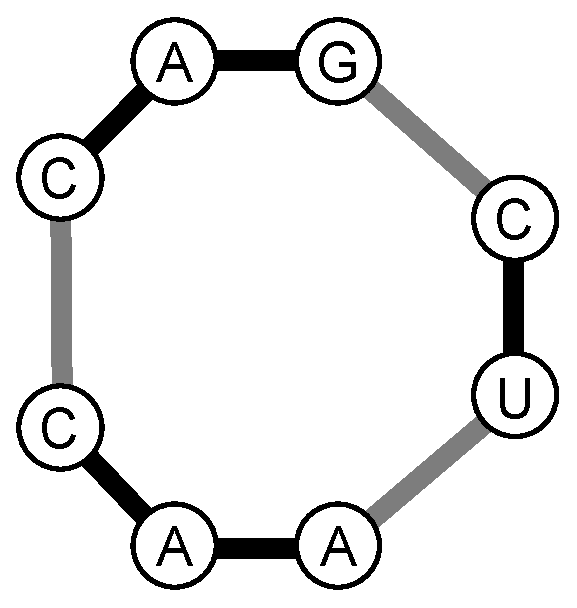
\includegraphics[scale=0.25]{CAGCUAAC-multiloop.eps}}}
  \right ) = 3.4 + 0*3 + 0.4*2 = 4.2 \text{ kcals/mol}.
\end{align}

If we sum up the contributions, we get that $\Delta G = -6.36 \text{
  kcals/mol}$. The energy of the MFE state can be computed using
software, and I find it to be $-3.06$ with just the first stem and a
large hairpin. [TODO: figure out what is wrong, make ct file, find energy].

\section{Critique of the Energy Model}

The energy model of RNA is not perfect, notably so. It is complex,
there are linear models, non-linear models, lookup tables, and
bonuses. Complexity is a very undesirable quality for a model, it
makes it hard to implement and hard for new researchers to get started
in the field.  Not only that, but many parameters have very high
error. For example, the initialization penalty for hairpin loops is
supposed to be different for different hairpin lengths, but most of
the terms aren't even $1\sigma$ away from each other. Because of this,
it is not clear what advantage these extra parameters give, perhaps
they could be reduced to one, to simplify the model greatly. Another
problem is that the data of the original experiments has been lost, so
no one can take a closer look at how well the parameters fit, and no
one seems to be interested in running the experiments again. The only
thing that seems to keep the current parameters in good standing is
relatively solid results in prediction, with something like 80\% of
base pairs correctly predicted. However, to make any progress from
this point, it is essential to get the energy model correct. 

If there was a list of big problems to tackle in RNA secondary
structure prediction, fixing the energy model should be a top
priority. The new model should be consistent and physically based and
confirmed by experiments. Some groups have made progress on creating
energy models for multi-loops that may perform better than the current
parameters [TODO: insert aalberts plug]. However, none of these
changes have been implemented in the software packages that currently
hold the grand majority of the secondary structure prediction
market. There are reasons for this, including the fact that the
software is massive, complicated, and poorly documented. Perhaps a new
energy model could usher in a better software framework for RNA
prediction that has:

\begin{enumerate}
\item Better naming conventions, with function, variable, and source
  file names describing precisely what they represent,
\item Consistently documented source files, perhaps with a full manual
  created with doxygen,  
\item Simpler energy models, with less branching and complexity.
\end{enumerate}

This is not to belittle the efforts of those that implemented Unafold
and RNAStructure, after all they accomplished the great feat of
implementing these complex software suites. Instead, it is to note
that the job is not done, and the items listed above are things that
need to be accomplished.

\section{Applications of RNA Structure Prediction}

RNA Secondary structure has many clinical applications including in
sequence design.

[TODO: finish this section]



%% This is an example first chapter.  You should put chapter/appendix that you
%% write into a separate file, and add a line \include{yourfilename} to
%% main.tex, where `yourfilename.tex' is the name of the chapter/appen
dix file.
%% You can process specific files by typing their names in at the 
%% \files=
%% prompt when you run the file main.tex through LaTeX.
\chapter{Partition Function Computation and Improvements}
\section{Introduction}

The partition function for a thermodynamic system of fixed volume, in
contact with a heat reservior with absolute temperature $T$, is
\begin{equation} Z = \sum_s e^{-E(s)/ RT }, \end{equation}
where $s$ denotes a particular state of the system, $E(s)$ is the
energy of that state, and $RT$ is the gas constant multiplied by the
temperature, specified above. Each particular term in the sum is
called that state's Boltzmann factor. The probability of a state is
then said to be its Boltzmann factor divided by the partition
function, or
\begin{equation} P(s) = \frac{1}{Z}e^{-E(s)/RT}.  \end{equation}
In our model an RNA strand is such a thermodynamic system, its
secondary structure is its state, and the rest of the cell is the
reservoir of heat. We assign each secondary structure an energy
according to the free energy model described in Chapter 1. According
to this model, the energy of a secondary structure is the sum of the
energies of its loops. 

To compute the partition function we must sum up every possible
secondary structure. There are many possible secondary structures, on
the order of $1.8^n$ where $n$ is the sequence length. However, the
computation of the partition function benefits greatly from the linear
nature of the energy model: it allows us to recursively define the
partition function. For example, say we have computed the full
partition function of a strand of $n$ bases, define a function $Q$
such that:
\begin{equation}
Q(i, j) = \text { sum of boltzmann factors for every structure contained between } i \text{ and } j.
\end{equation}
The full partition computation can therefore be represented as the
function $Q$ acting on the bounding two bases $1$ and $n$: 
\begin{equation}
 Q(1, n) = \sum_{s \text{ on } [1,n]} e^{-E(s)/RT}.
\end{equation}
If we now extend the strand by attaching a small hairpin to the end,
as pictured in Figure \ref{fig:attachedHairpin}, there is no need to
go back and recompute the energy of every single secondary structure,
rather we can just multiply the already-computed partition function by
the boltzmann factor of the hairpin turn (let $E(h)$ be the hairpin
energy) to get the new partition function:
\begin{figure}[h]
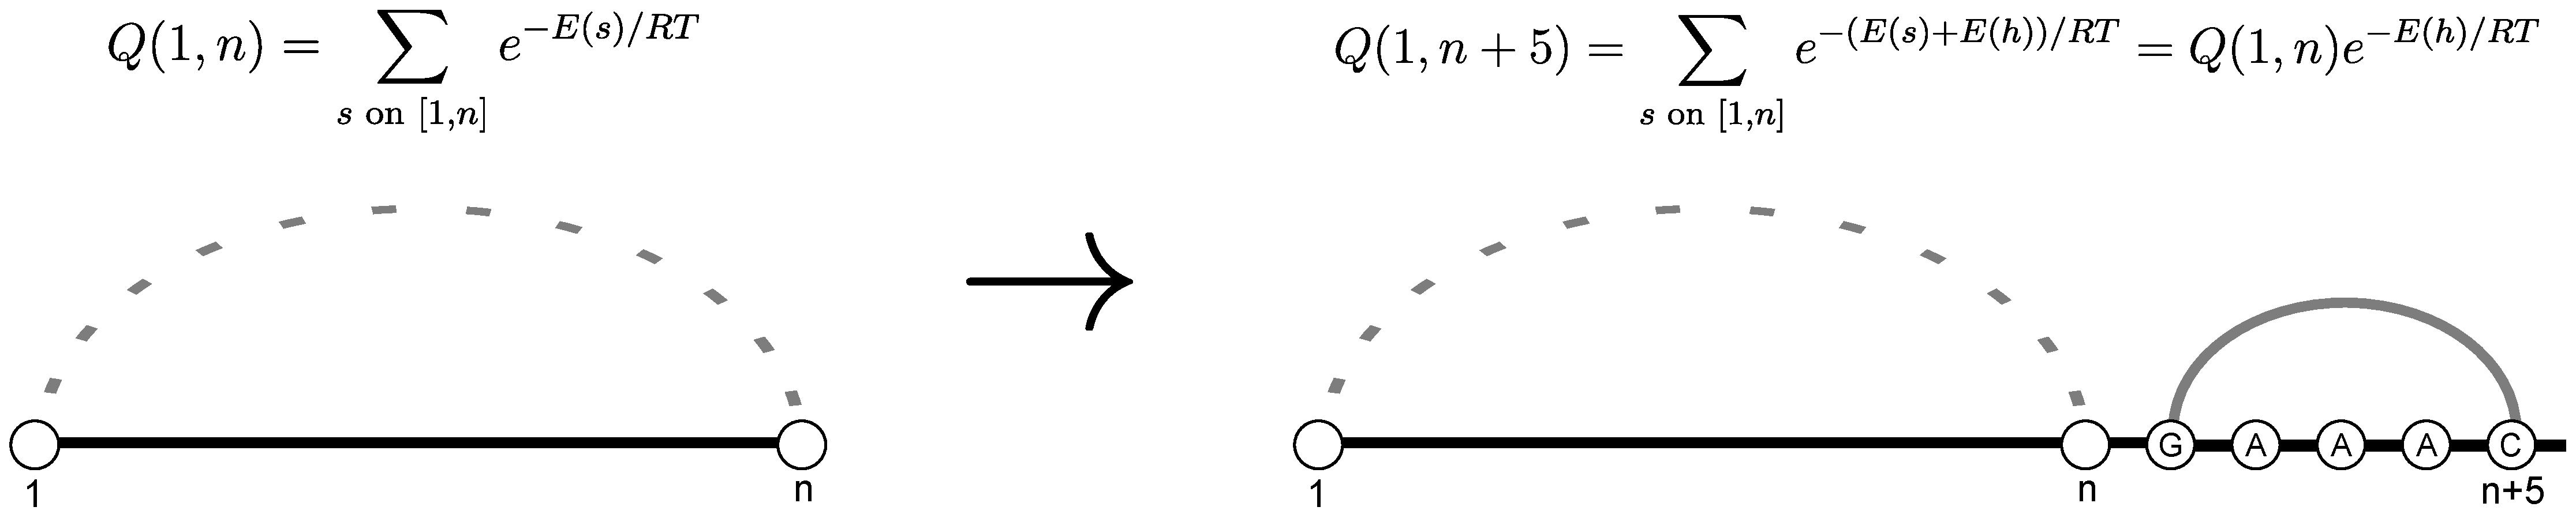
\includegraphics[width=\textwidth]{attachedHairpin.eps}
\caption{Extending the strand by adding an attached hairpin adds the
  energy of the hairpin to each structure. To compute the new
  partition function $Q(1, n+5)$, we do not need to sum the energies
  of all possible structures again, we can simply use the old value,
  $Q(1,n)$, and multiply it by the Boltzmann factor of the
  hairpin. This is the concept behind the dynamic programming
  algorithm.}
\label{fig:attachedHairpin}
\end{figure}
\begin{equation}
Q(1, n + 5) = \sum_{s \text{ on } [1,n]} e^{-(E(s) + E(h))/RT} = Q(1, n)e^{-E(h)/RT}. 
\end{equation}
This replaces an exponential-time computation (the sum), with a
constant time computation (multiplying the pre-computed $Q(1, n)$ with
the energy term). In general, this technique allows us to compute the
partition function efficiently, working up from $Q(1, 2)$ to
$Q(1,n)$. In computer science this technique is called dynamic
programming, a fancy name for the technique of storing the
results of a computation in a table for later use.

The dynamic programming algorithm for computing the partition function
of an RNA strands has several versions, depending on how in depth you
go with the energy model. The simplest algorithms allow for only
structures with nested base pairs. Nested means that the structure can
be represented with the parenthesis, for example
(((..((((....))))(((..)))..))), or without crossing pairs in expanded
loop diagrams such as the ones in Figure
\ref{fig:attachedHairpin}. Note that this kind of structure excludes
pseudoknots.  If you ignore psuedoknots, which is standard in the
field, and if you make an approximation that internal loops will never
exceed a certain length, the fastest algorithm runs in $O(n^3)$. We
believe that we can streamline this computation even more, taking
advantage of the fact that empirically, the number of probable base
pairs of a strand of length $n$ seems to grow like $n$, not
$n^2$. This is the same result we used to speed up the stochastic
traceback algorithm and potentially a partition function algorithm
that includes pseudoknots. The algorithm will be presented in its
simplest form, with more complicated versions available in the
appendices.

\section{Motivation}

In certain situations, such as partition function clustering, the
partition function is computed and recomputed several times. If the
partition function takes on the order of hours or days to compute,
this can make partition function clustering a bad option. However in
these situations it is also true that the partition function is
recomputed with almost the same properties, just certain pairs
restricted. This motivates a method of computing the partition
function using a known pairs heueristic to prune away unneccesary
computation.

This concept has already been implemented to great success in the
stochastic traceback algorithm. We've been able to show via experiment
that the partition function only admits roughly $O(n)$ pairs with
probabilities above thresholds around the machine precision limit. If
we have the partition function already computed, we can recompute it
by only adding in pairs that have sufficient probability. We can also
extend this method: if a good heuristic appears in the future, one
that can eliminate a large number of pairs, while being
computationally cheap, we should be able to use the results to speed
up the partition function computation.

\section{Computation}

The standard way of computing the partition function involves filling
out a table where the $(i,j)$ member represents the partition function
for the substrand from base $i$ to base $j$. Because the energy model
for RNA is (mostly) linear, the partition function from $i$ to $j$ can
be expressed as a function of nearby members of this table. This
function is the recurrence relation for the partition function of
RNA. Because the free energy model is so complicated and has gone
through many iterations, differenct RNA folding software packages
implement different versions of the recurrence relation, and they vary
widely in complexity.

The definitive representation of the recurrence relation for RNA was
formulated in 1990 by J.S. McCaskill in his landmark paper \emph{The
Equilibrium Partition Function and Base Pair Binding Probabilities for
RNA Secondary Structure} [TODO: cite?]. The formula is also presented
better and explained well by a later paper by Dirks and Pierce in 2003
(Dirks \& Peirce 2003). Starting at the outermost layer of this
relation, the formula for the partition function of the strand from
base $i$ to base $j$ is:

\begin{equation} Q(i,j) = 1 + \sum_{i \leq d < e \leq j}Q(i, d - 1)
Q^b(d, e) \end{equation}

The theory behind this formula is that the partition function is a sum
of the empty state (the first term, 1) and the state with at least 1
pair, the furthest pair to the right being pair $(d,e)$. The term
$Q^b(d,e)$ is the partition function assuming that base $d$ and base
$e$ are paired. This function has the following recursion relation:

\begin{equation} Q^b(i, j) = e^{-\frac{\text{Hairpin}(i,j)}{RT}} +
\sum_{i \leq d < e \leq j} e^{\frac{\text{Interior}(i, d, e,
j)}{RT}}Q^b(d,e) + \sum_{i \leq d < e \leq j} Q^m(i + 1, d - 1)Q^b(d,
e) e^{-\frac{\alpha_1 + 2\alpha_2 + \alpha_3(j-e-1)}{RT}}
\end{equation}

The theory behind this formula is that the partition function for a
strand assuming $i$ and $j$ are paired includes 3 cases:

\begin{enumerate}

\item

There are no bases paired between $i$ and $j$, the loop is a hairpin
and uses the energy function for a hairpin loop, we call
$\text{Hairpin}(i,j)$, which consists of data table lookups.

\item There is an internal loop between $i$ and $j$ and a second pair
$d$ and $e$. This uses a different energy model, we call
$\text{Internal}(i,j)$ and also consists of data table lookups.

\item There is a multiloop formed by the pair $i$ and $j$, which must
be carefully accounted for using a special model for multiloops.

\end{enumerate}

The multiloop partition function, $Q^m(i, j)$ is the last piece of the
puzzle. The formula is:

\begin{equation} Q^m(i, j) = \sum_{i \leq d < e \leq j}
e^{-\frac{\alpha_2 + \alpha_3(d-i) + \alpha_3(j-e)}{RT}} Q^b(d,e) +
Q^m(i, d - 1)Q^b(d, e) e^{-\frac{\alpha_2 + \alpha_3(j-e)}{RT}}
\end{equation}

In english, this just means we sum up all the ways to just have 1
pair, and then all the ways to have more than one pair. The case with
no pairs is not included, as in the original recursion in $Q^b$,
$Q^m(i+1, d-1)Q^b(d,e)$ must yield at least 2 pairs. Since $Q^b$ makes
one, then $Q^m$ must make at least 1.

For example, the UNAFold software package implements a particularly
hairy recurrence relation. Define $Q(i,j)$ as the partition function
from $i$ to $j$, $Q'(i,j)$ to be the partition function from $i$ to
$j$, assuming $i$ and $j$ are paired, and define $Q^1(i,j)$ to be the
partition function from $i$ to $j$, assuming exactly 1 pair happens on
that interval, and that pair happens with base $i$. The recurrence
relation is therefore

[recurrence relation]

Note the terms $Z_{ND}$, $Z_{3'D}$, $Z_{5'D}$, and $Z_{DD}$ are extra
free energy terms corresponding to 'dangle energies' which are the
results of an experiment later implemented in the model to improve it
from the standard energy model. In addition there are AU penalty terms
appended to where pairs are made, as AU and GU pairs have penalties
associated with forming. These additional energy terms improve the
model's predictive ability and bring the model closer to the "truth",
however it unfortunately makes the partition function seem very
threatening.

Our new partition function relation has the following theory behind
it: Assume we have the functions $I : B \to \{B\}$ and $J : B \to
\{B\}$ that return the set of all probably pairs for a base $i$ or a
base $j$, respectively. The recurrence relation can be reformulated in
the following way:

\section{Derivation of new Q(i, j) formula}

In UNAfold, we have that the old recurrence relations were as follows:

\begin{equation}
Q(i,j) = \sum_{k=i}^j \left ( Q(i, k-1) + e^{-\frac{b(k-i)}{RT}}  \right )Q^1(k, j)
\end{equation}
where 
\begin{equation}
\begin{split}
Q^1(i, j) = \ \ & Q^1(i, j - 1) e^{-\frac{b}{RT}}  \\
 +\ & e^{-\frac{c}{RT} }Z_{ND}(i, j) Q'(i, j)  \\
+\ & e^{-\frac{b + c}{RT}}Z_{5'D}(i + 1, j)Q'(i + 1, j)  \\
+\ &  e^{-\frac{b + c}{RT}}Z_{3'D}(i, j-1)Q'(i, j - 1)  \\
+\ &  e^{-\frac{2b + c}{RT}}Z_{DD}(i + 1, j-1)Q'(i + 1, j-1) 
\end{split}
\end{equation}
\noindent
We can expand the recursive definition of $Q^1(i,j)$:

\begin{equation}
\begin{split}
Q^1(i, j) = \sum_{k' = i + 1}^j e^{-\frac{b(j - k')}{RT} } \bigg [ \ 
  & e^{-\frac{c}{RT} }Z_{ND}(i, k') Q'(i, k') \\
 +\ & e^{-\frac{b + c}{RT}}Z_{5'D}(i + 1, k')Q'(i + 1, k') \\ 
+\  & e^{-\frac{b + c}{RT}}Z_{3'D}(i, k'-1)Q'(i, k' - 1) \\
+\  & e^{-\frac{2b + c}{RT}}Z_{DD}(i + 1, k'-1)Q'(i + 1, k'-1) \   \bigg ]
\end{split}
\end{equation}
\noindent
Plugging this into $Q(i,j)$ we get:

\begin{equation}
\begin{split}
Q(i, j) = \sum_{k= i}^j\ \sum_{k' = k + 1}^j \left (  Q(i, k-1) + e^{-\frac{b(k-i)}{RT}} \right ) e^{-\frac{b(j - k')}{RT} } \bigg [ \ 
  & e^{-\frac{c}{RT} }Z_{ND}(k, k') Q'(k, k')  \\
+\  & e^{-\frac{b + c}{RT}}Z_{5'D}(k + 1, k')Q'(k + 1, k') \\ 
+\ & e^{-\frac{b + c}{RT}}Z_{3'D}(k, k'-1)Q'(k, k' - 1) \\
+\  & e^{-\frac{2b + c}{RT}}Z_{DD}(k + 1, k'-1)Q'(k + 1, k'-1) \   \bigg ]
\end{split}
\end{equation}
\noindent
Now we'll take the $j$th element of the second sum and split it out (note that the $j$th part of the 1st sum has no elements to sum now, so we can decrement that too):
\begin{equation}
\begin{split}
Q(i, j) = \sum_{k= i}^{j-1}\ \sum_{k' = k + 1}^{j-1} \left (  Q(i, k-1) + e^{-\frac{b(k-i)}{RT}} \right ) e^{-\frac{b(j - k')}{RT} } \bigg [ \ 
  & e^{-\frac{c}{RT} }Z_{ND}(k, k') Q'(k, k')  \\
+ \  & e^{-\frac{b + c}{RT}}Z_{5'D}(k + 1, k')Q'(k + 1, k')\\ 
+\   & e^{-\frac{b + c}{RT}}Z_{3'D}(k, k'-1)Q'(k, k' - 1) \\
+\  & e^{-\frac{2b + c}{RT}}Z_{DD}(k + 1, k'-1)Q'(k + 1, k'-1) \   \bigg ] \\
+\ \sum_{k=i}^j  \left (  Q(i, k-1) + e^{-\frac{b(k-i)}{RT}} \right ) \bigg [ \ 
  & e^{-\frac{c}{RT} }Z_{ND}(k, j) Q'(k, j) \\
+\  & e^{-\frac{b + c}{RT}}Z_{5'D}(k + 1, j)Q'(k + 1, j) \\ 
+\  & e^{-\frac{b + c}{RT}}Z_{3'D}(k, j-1)Q'(k, j - 1) \\
 +\  & e^{-\frac{2b + c}{RT}}Z_{DD}(k + 1, j-1)Q'(k + 1, j-1) \   \bigg ]
\end{split}
\end{equation}
\noindent
Notice that the double sum is simply $Q(i,j-1)e^{-b/RT}$ and the terms of the second, single sum are over the pairs with $j$ or $j-1$. Therefore, we can use our heuristic for the pairs of $j$ and $j-1$ to produce the following computation for $Q(i, j)$ which is much more efficient than the previous ones:
\begin{equation}
\begin{split}
Q(i,j) = Q(i, j-1)e^{-b/RT} +  \sum_{k(j)} & \bigg [  \left (  Q(i, k-1) + e^{-\frac{b(k-i)}{RT}} \right ) \
   e^{-\frac{c}{RT} }Z_{ND}(k, j) Q'(k, j)  \\
+\ & \left (  Q(i, k-2) + e^{-\frac{b(k-i-1)}{RT}} \right )    e^{-\frac{b + c}{RT}}Z_{5'D}(k, j)Q'(k, j) \   \bigg ]  \\
+\  \sum_{l(j-1)} & \bigg [  \left (  Q(i, l-1) + e^{-\frac{b(l-i)}{RT}} \right ) \
   e^{-\frac{c}{RT} }Z_{ND}(l, j-1) Q'(l, j-1)  \\
+\ & \left (  Q(i, l-2) + e^{-\frac{b(l-i-1)}{RT}} \right )   e^{-\frac{2b + c}{RT}}Z_{DD}(l, j-1)Q'(l, j-1) \   \bigg ] 
\end{split}
\end{equation}

\section{Derivation of new Q'(i, j) formula}
For $Q'(i, j)$ we start with the recursion:

\begin{equation}
\begin{split}
Q'(i,j) = Z_H(i, j) &+ Z_S(i, j) Q'(i+1, j-1) + QBI(i, j) \\
+\ & e^{-\frac{a+c}{RT}}Z_{ND}(j, i) \sum_{k = i + 3}^{j-5}Q(i+1, k - 1)Q^1(k, j-1)  \\
+\ & e^{-\frac{a+b+c}{RT}}Z_{3'D}(j, i) \sum_{k = i + 4}^{j-5}Q(i+2, k - 1)Q^1(k, j-1)  \\
+\ & e^{-\frac{a+b+c}{RT}}Z_{5'D}(j, i) \sum_{k = i + 3}^{j-6}Q(i+1, k - 1)Q^1(k, j-2) \\
+\ & e^{-\frac{a+2b+c}{RT}}Z_{DD}(j, i) \sum_{k = i + 4}^{j-6}Q(i+2, k - 1)Q^1(k, j-2) 
\end{split}
\end{equation}
\noindent
The 4 for loops in this make this an expensive computation as the number of bases gets very high. However, these for loops are very similar to the partition function in structure. Indeed, we could perhaps replace each of them with a function of the form $Q^m(i, j)$ defined as

\begin{equation}
Q^m(i, j) = \sum_{k = i +3}^{j-5} Q(i + 1, k - 1) Q^1(k, j - 1)
\end{equation} 
\noindent
Which would simplify the previous sum to a constant time computation, provided we have memoized $Q^m$:
\begin{equation}
\begin{split}
Q'(i,j) = Z_H(i, j) &+ Z_S(i, j) Q'(i+1, j-1) + QBI(i, j)  \\
+\ & e^{-\frac{a+c}{RT}}Z_{ND}(j, i) Q^m(i, j)  \\
+\ & e^{-\frac{a+b+c}{RT}}Z_{3'D}(j, i) Q^m( i + 1, j) \\
+\ & e^{-\frac{a+b+c}{RT}}Z_{5'D}(j, i) Q^m(i, j- 1) \\
+\ & e^{-\frac{a+2b+c}{RT}}Z_{DD}(j, i) Q^m(i + 1, j -1)
\end{split}
\end{equation}

\noindent
Now there just needs to be a way to efficiently compute $Q^m$. First we substitute in the expanded version of $Q^1$:

\begin{equation}
\begin{split}
Q^m(i, j) = \sum_{k = i + 3}^{j - 5}\  \sum_{k' = k + 1}^{j- 1} Q(i + 1, k - 1)  e^{-\frac{b(j - k')}{RT} } \bigg [ \ 
  & e^{-\frac{c}{RT} }Z_{ND}(k, k') Q'(k, k') \\
+\  & e^{-\frac{b + c}{RT}}Z_{5'D}(k + 1, k')Q'(k + 1, k') \\ 
 +\ & e^{-\frac{b + c}{RT}}Z_{3'D}(k, k'-1)Q'(k, k' - 1) \\
+\  & e^{-\frac{2b + c}{RT}}Z_{DD}(k + 1, k'-1)Q'(k + 1, k'-1) \   \bigg ]
\end{split}
\end{equation}

\noindent
Then we do as before and seperate out the $j$th term of the second sum. Note that there seems to be an additional sum needed to account that I've decreased the first sum's endpoint to $j-6$, but the sum ends up being from $k'= j-4$ to $k' = j -2$ and since $Q'$ for bases less than 4 apart is 0 due to hairpin loop rules, this sum is equal to zero.
\begin{equation}
\begin{split}
Q^m(i, j) = \sum_{k = i + 3}^{j - 6}\  \sum_{k' = k + 1}^{j- 2} Q(i + 1, k - 1)  e^{-\frac{b(j - k'-1)}{RT} } \bigg [ \ 
  & e^{-\frac{c}{RT} }Z_{ND}(k, k') Q'(k, k') \\
+ \  & e^{-\frac{b + c}{RT}}Z_{5'D}(k + 1, k')Q'(k + 1, k') \\ 
+ \  & e^{-\frac{b + c}{RT}}Z_{3'D}(k, k'-1)Q'(k, k' - 1) \\
 + \  & e^{-\frac{2b + c}{RT}}Z_{DD}(k + 1, k'-1)Q'(k + 1, k'-1) \   \bigg ]\\
+ \ \sum_{k = i + 3}^{j - 5}\ Q(i + 1, k - 1)  \bigg [ \ 
  & e^{-\frac{c}{RT} }Z_{ND}(k, j-1) Q'(k, j-1)  \\
+ \  & e^{-\frac{b + c}{RT}}Z_{5'D}(k + 1, j-1)Q'(k + 1, j-1) \\ 
  + \ & e^{-\frac{b + c}{RT}}Z_{3'D}(k, j-2)Q'(k, j-2)\\
+ \  & e^{-\frac{2b + c}{RT}}Z_{DD}(k + 1, j-2)Q'(k + 1, j-2) \   \bigg ]\ 
\end{split}
\end{equation}
\noindent
The double sum is again going to be equal to $Q^m(i, j -1)e^{-b/RT}$, and the second sum can be made much more efficient by our heuristic. 
\begin{equation}
\begin{split}
Q^m(i, j) = Q^m(i, j - 1)e^{-b/RT} + \sum_{k(j - 1)} \bigg [ & Q(i + 1, k - 1)   
  e^{-\frac{c}{RT} }Z_{ND}(k, j-1) Q'(k, j-1)  \\
 + \ &Q(i + 1, k - 2) e^{-\frac{b + c}{RT}}Z_{5'D}(k, j-1)Q'(k, j-1)  \bigg ]\ \\
+ \sum_{k(j-2)} \bigg [ & Q(i + 1, k - 1)   
  e^{-\frac{c}{RT} }Z_{3'D}(k, j-2) Q'(k, j-2)  \\
  +\ &Q(i + 1, k - 2) e^{-\frac{b + c}{RT}}Z_{DD}(k, j-2)Q'(k, j-2)  \bigg ]
\end{split}
\end{equation}
\noindent

Since the $k$s for any individual $j$ are found to be quite limited, the final form should be much more efficient at computing the $Q'(i, j)$.

Note that for $Q$ and in many places for $Q'$, instead of a sum over
the known $k$ that could possibly begin a leftmost pair, we see a
double sum. One of them over $k$ that could end a leftmost pair, and
this sum is limited to a certain length below $j$. This is just making
the same assumption that the internal loop computation makes: there
are not arbitrarily long strands without base pairs, after a certain
number of bases it becomes overwhelmingly more likely to make a base
pair that we can virtually ignore the energy of the the cases of
length beyond a certain $L$.

As for the seocnd sum, since the number of probable pairs for a base
$i$ has been shown empirically to be roughly constant, regardless of
length, the second sum is essentially constant. What this all means is
that all $O(n^2)$ computations of $Q(i,j)$'s are roughly constant
time. This means that the overall algorithm is $O(n^2)$, an
improvement over the previous algorithms asymptotic bound by and order
of $n$!



\section{Results}

[TODO: include timing plots for new partition function]

Calculating the partition function is still difficult, but it can be
improved in the asymptotic case. The results show that the new
computation has a large constant factor in the beginning of the
algorithm. This could be related to the way the internal loop
partition function is calculated, where we still have an $O(n^3)$
algorithm until the number of nucleotides is greater than 30. This
effect is relatively diminished as we get into the 1000s in term of
base count, but it still is a large constant factor. As we increase
the probability barrier, we get further reductions in runtime.

[TODO: include plot with different times for different probability
thresholds]

A large part of the verification of an improved algorithm is showing
that it produces acceptable results compared to the old algorithm, as
you can see in the plot, our algorithm gives the same results up to 1
part in 1 million [TODO: check this]. Increasing the probability
threshold changes the results by [TODO: find out].

[TODO: include plot of verification]

\section{Conclusion}

The partition function computation is hard and is a limiting factor in
RNA structure prediction. However, given a heuristic to predict the
base pairs, we can make the algorithm run faster. These improvements
can be used in applications such as clustering based on our nestedness
measure, using the partition function. These improvements also open up
several possible branches for further investigation. Can a heuristic
be generated before the partition function is computed, so that the
pairs can be restricted and the computation done in much faster time
than the $O(n^3)$ algorithm? Could this concept be applied to the
pseudoknot algorithm to possibly speedup the computation for that as
well? Applications of this sort could have tremendous impact on RNA
secondary structure prediction, opening up incredible avenues of
potential.


%% This is an example first chapter.  You should put chapter/appendix that you
%% write into a separate file, and add a line \include{yourfilename} to
%% main.tex, where `yourfilename.tex' is the name of the chapter/appendix file.
%% You can process specific files by typing their names in at the 
%% \files=
%% prompt when you run the file main.tex through LaTeX.
\chapter{Stochastic Traceback Algorithm and Improvements}

\section{Introduction}

The stochastic traceback algorithm was introduced by Ye Ding and
Charles Lawrence \cite{ding2003statistical} as a means to explore the
energy landscape of RNA by sampling structures according to their
Boltzmann probabilities. This was important because the minimum free
energy structure was very sensitive to errors in the parameters of the
free energy model, and although algorithms existed for generating
suboptimal structures, they either sampled a very limited set of
states \cite{zuker1989finding}, or had exponential runtime and the
output did not have the same distribution as the physical ensemble of
states \cite{wuchty1999complete}. Structures sampled according to this
algorithm can be clustered into macrostates.

The method first computes the partition function, then it ``traces
back'' over the contents of the tables calculated during that
algorithm. Specifically, the tables $Q(i,j)$, $Q^b(i,j)$, etc. now
contain information about the conditional probabilities of bases
pairing. Starting from a bare, undetermined strand at the top of the
recurrence relations, the stochastic traceback samples pairs between
bases until a structure is formed such that its probability of it
being created by the algorithm is equal to its Boltzmann weight
$e^{-E(s)/RT}/Z$.

The general principle of the backwards trace is that,
presented with several possibilities for the structure along a
sequence from $i$ to $j$, the sampling probability for a case is the
contribution to the partition function by that case's partition
function. For example, since the partition function $Q(i, j)$ is defined:
\begin{equation}
Q(i,j) = \overbrace{e^{-b(j-i+1)/RT}}^{\text{empty}} + \overbrace{\sum_{\substack{ d,e \\ i \leq d < e \leq j}}Q(i, d - 1) Q^b(d, e) e^{-b(j-e)/RT}}^{\text{rightmost pair}},
\end{equation}
during a stochastic traceback the probability of sampling a pairless
strand, and the probability of drawing a rightmost pair $(d,e)$ and
recursing from there are:
\begin{align}
P(\text{empty} | i, j) &= \frac{e^{-b(j-i+1)/RT} }{Q(i,j)} \\ 
P(\text{pair } (d,e) | i, j ) &= \frac{ Q(i, d-1) Q^b(d,e) e^{-b(j-e)/RT}}{Q(i,j)}. 
\end{align}
Notice that when summed together for every possible case of $(d,e)$,
the numerator becomes the definition of $Q(i,j)$, so these
probabilities are naturally normalized. Likewise, since $Q^b(i,j)$ is
defined as 
\begin{equation}
\begin{split}
 Q^b(i, j) =& \overbrace{e^{-E_h(i,j)/RT}}^{\text{hairpin}} +
 \overbrace{e^{-E_s(i, j)/RT} Q^b(i+1, j-1)}^{\text{stack}} \\ 
& + \overbrace{\sum_{\substack{d,e \\ i < d< e< j}} e^{-E_i(i, d, e, j)/RT}Q^b(d,e)}^{\text{internal}} \\ 
& + \overbrace{e^{-a/RT} \sum_{\substack{d,e \\ i < d< e< j}} Q(i+1, d-1) Q^b(d,e) e^{-b(j-e-1)/RT}}^{\text{multiloop}}.
\end{split}
\end{equation}
The probability of sampling a hairpin, stack loop, internal loop, and multiloop are:
\begin{align}
P(\text{hairpin} | i, j) &= \frac{ e^{-E_h(i,j)/RT} } { Q^b(i,j) } \\
P(\text{stack} | i, j ) &= \frac{ e^{-E_s(i,j)/RT} Q^b(i+1, j-1) } {Q^b(i,j)}  \\
P(\text{internal } (d, e) | i, j) &= \frac{e^{-E_i(i, d, e, j)/RT} Q^b(d,e)}{Q^b(i,j) }\\
P(\text{multi }(d,e) |i, j ) &= \frac{ e^{-a/RT} Q(i + 1, d-1) Q^b(d,e) e^{-b(j-e-1)/RT} } { Q^b(i,j)} 
\end{align}
Notice for the same reason as before, all the probabilities for the
$Q^b$ recursion sum to one. In general, the stochastic traceback can
be readily understood by examining the recurrence relation figures
from chapter 2: Figure \ref{fig:recurrenceRelationsQij} and Figure
\ref{fig:recurrenceRelationsQbij}. We start at the $Q$ recursion for
the strand, we may pick a pair and add it to the structure, but in
general, for every pair added we recurse down to $Q^b$ on that region
to determine the structure below that pair. For every structure left
undetermined, we use the probabilities from $Q$ to determine that
structure and so on. 

\begin{figure}
\centering
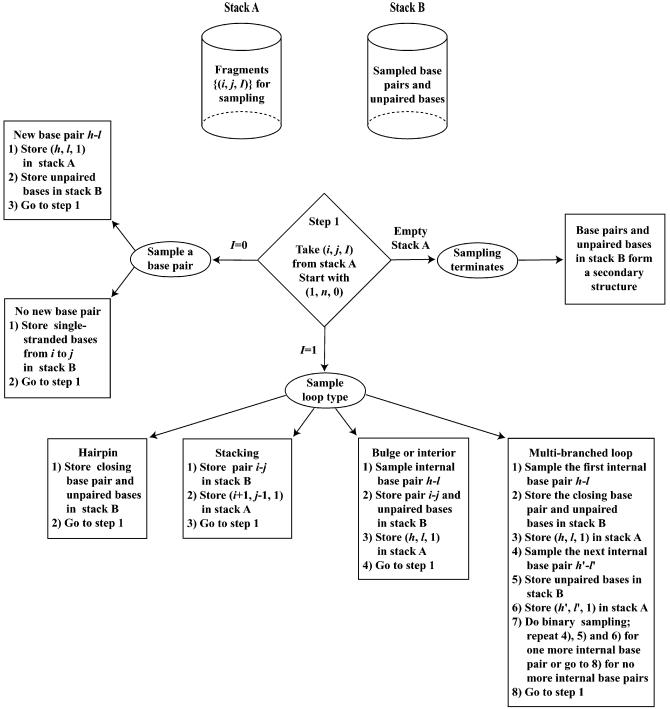
\includegraphics[width=\textwidth]{stochastic-alg-diagram.jpg}
\caption[Stochastic Traceback Flowchart]{Flowchart of the algorithm from Ding and Lawrence's paper
  \cite{ding2003statistical}. Basically: if we are on a $Q(i,j)$
  recursion, sample either an empty section or a rightmost pair. For
  $Q^b$ choose a loop type and corresponding pairs if
  applicable. After both cases recurse down appropriately so that
  $Q^b$ is drawn for any pair created and $Q$ for any open region.}
\label{fig:stoch-flowchart}
\end{figure}

The algorithm's implementation uses two stack data structures. A stack
can be thought of as a literal "stack", like papers stacked on a desk,
except instead of paper their are items of data. There are two basic
operations, one to put an item on the top of the stack, and another to
retrieve an item off the top. These are called "push" and "pop"
operations, respectively, in Computer Science. The data items we will
be pushing on to the first stack, A, are of the form $\{(i,j), b\}$
where $i$ and $j$ are indexes along the strand and $b$ is either
$true$ if we have determined that $i$ and $j$ are paired, or $false$
otherwise. The second stack, B, is where we'll collect pairs and
unpaired bases for one sample.

\begin{figure}[t]
\bfseries\small
The initialization of the algorithm is to push $\{(1, n), false\}$
onto the stack. From there the algorithm repeats the following steps:
\begin{enumerate}
\item Pop an element, $\{i, j, b\}$ off stack A.
\item Case b is $false$:
\begin{enumerate}
\item ($Q(i,j)$ recursion) Pick empty or pair $(k,l)$ with
  probabilities listed above. If empty, push all pairs on $[i, j]$
  inclusive onto B as unpaired bases, if not push $\{(d, e), true\}$
  and $\{(i, d-1), false\}$ onto A.
\end{enumerate}
\item Case b is $true$:
\begin{enumerate}
\item ($Q^b(i,j)$ recursion) Choose what type of loop $(i,j)$ is from
  the probabilities listed above.
\item Push the appropriate elements onto the stack for that loop type,
  see Figure \ref{fig:stoch-flowchart}.
\end{enumerate}
\item If stack A is empty, the pairs and unpaired bases in stack B
  become a sampled structure. Reinitialize for additional samples.
\end{enumerate}
\caption[Stochastic Traceback Pseudocode]{The stochastic traceback
  algorithm is implemented by pushing the recursive elements back onto
  the stack to sample a full structure. }
\label{fig:stochastic-pseudocode}
\end{figure}

The algorithm displayed in Figure \ref{fig:stochastic-pseudocode} is
what gets the job done. The probability of the structure is equal to
the product of the probabilities that determined its pairs and empty
regions, but if you follow the recursion all the way down you see that
this results in just the Boltzmann factor for the structure:
\begin{equation}
P(s) = \prod_{\text{cases}} \frac{P(\text{case})}{Q(\text{case})} =
\frac{1}{Z} e^{-E(s)/RT}.
\end{equation}

\section{Motivation}

In the past 10 years, the stochastic traceback algorithm has become an
increasingly central part of RNA secondary structure prediction
algorithms \cite{mathews2006revolutions}. This is because they present
many advantages over the minimum free energy prediction. It can be
shown that the minimum free energy state, even though it is the most
probable state, can still have astronomically unlikely probabilities
on average for typical strands of reasonable length (Figure
\ref{fig:probMFE}). The more important concept in understanding the
physical behavior of an RNA strand is therefore the overall shape of
the energy landscape. Although the probability of any individual
structure might be infinitesimally small, there can be shown to be
relatively few large basins containing clusters of similar foldings.
The consensus structures and the difference between the consensus
structures of these basins define the function of the RNA molecule.

The way the stochastic algorithms probe that is by providing
structures to group into these basins, and since the stochastic
traceback algorithm samples states with the exact probability defined
by the partition function, we know that the macrobehavior of these
samples match what we would probably see in reality. There is one
catch and that is statistical error. However, the error can be reduced
and the landscape can be further explored the more stochastic samples
we make.

The need to sample large numbers of secondary structures makes a
speedup very convenient, and that is what motivates our current
expedition.

\section{Adding Efficiency}

Taking advantage of the empirical fact that the number of probable
base pairs for an RNA strand tend to grow very slowly, we can restrict
our traceback to only explore bases that we know can pair with one
another. This is as simple as replacing the old recurrence relations
with the new ones. For example during a $Q(i,j)$ state of the
recursion there would be probabilities of:
\begin{align}
P(\text{empty} | i, j) &= \frac{e^{-b(j-i+1)/RT}}{Q(i,j)}\\
P(\text{goto } Q^m | i, j) &= \frac{Q^m(i, j) }{Q(i, j) }.
\end{align}
For a $Q^m$ state:
\begin{align}
P(\text{continue} | i, j) = \frac{Q^m(i, j -1) e^{-b/RT}} {Q^m(i, j) }\\
P(\text{pair } (k, j) | i, j) = \frac{Q(i, k - 1) Q^b(k, j) } {Q^m(i,j) }.
\end{align}
And finally for $Q^b(i, j)$:
\begin{align}
P(\text{hairpin} | i, j) &= \frac{ e^{-E_h(i,j)/RT} } { Q^b(i,j) } \\
P(\text{stack} | i, j ) &= \frac{ e^{-E_s(i,j)/RT} Q^b(i+1, j-1) } {Q^b(i,j)}  \\
P(\text{internal } (d, e) | i, j) &= \frac{e^{-E_i(i, d, e, j)/RT} Q^b(d,e)}{Q^b(i,j) }\\
P(\text{goto } Q^m |i, j ) &= \frac{ e^{-a/RT} Q^m(i,j) } { Q^b(i,j)}. 
\end{align}


\section{Results} 

As one can see from Figure \ref{fig:stochOvN}, the speedup is
enormous. For randomly sampled sequences up to lengths in the
thousands, the old stochastic timing grows quadratically, while the
new method flat-lines below it. The log-log plot in Figure
\ref{fig:stochLogLog} shows that the algorithm is not quite $O(n)$,
this is probably because there is a probability to recurse down
different cases of $Q^m$, however it is still quite below the old
slope.
\begin{figure}[t]
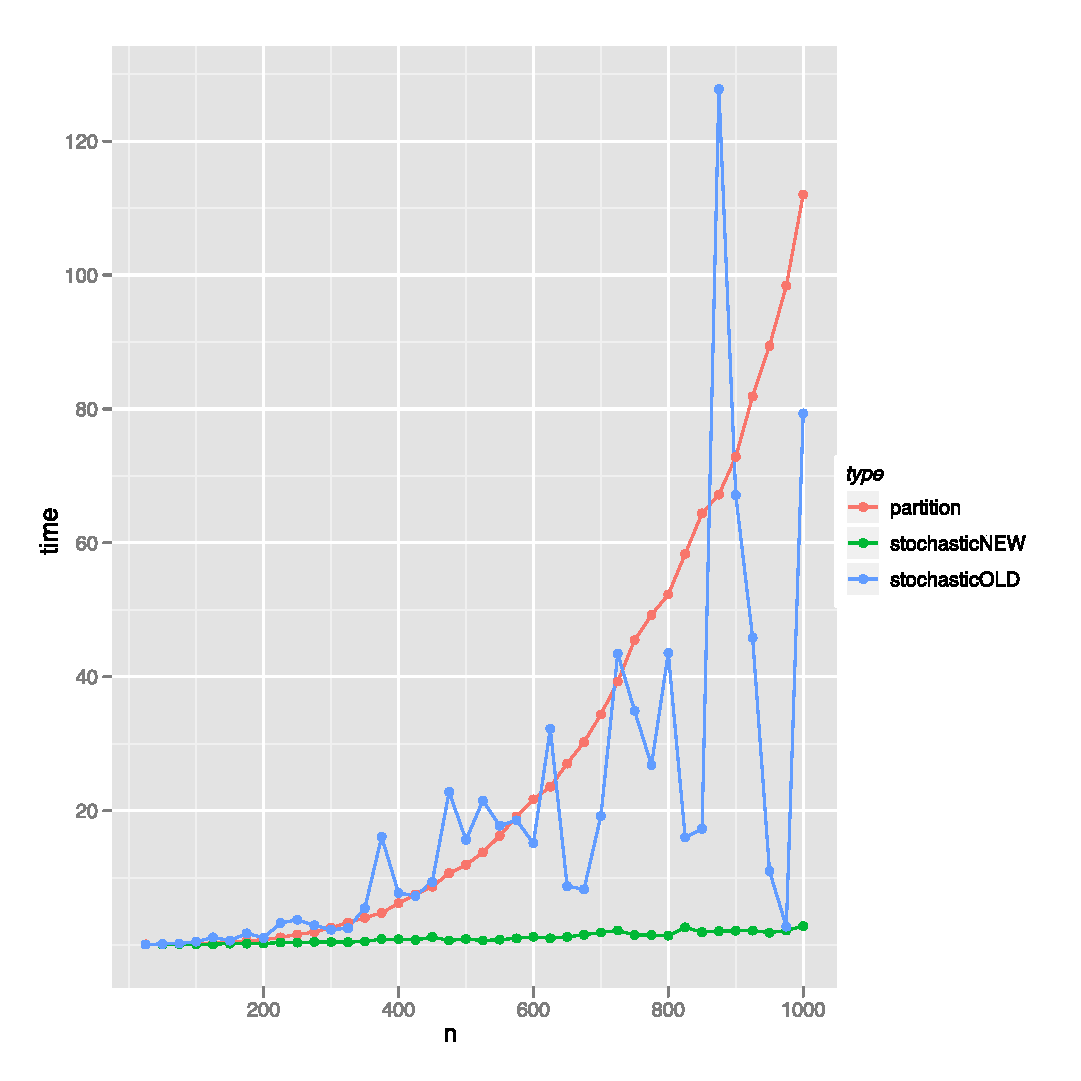
\includegraphics[width=\textwidth]{stochOldvNew.eps}
\caption[Stochastic Traceback Speedups]{A comparison of the
  computation time between the partition function computation, and
  stochastic tracebacks of 1000 samples with the Old algorithm and the
  new algorithm. The new algorithm is much faster.}
\label{fig:stochOvN}
\end{figure}
\begin{figure}[t]
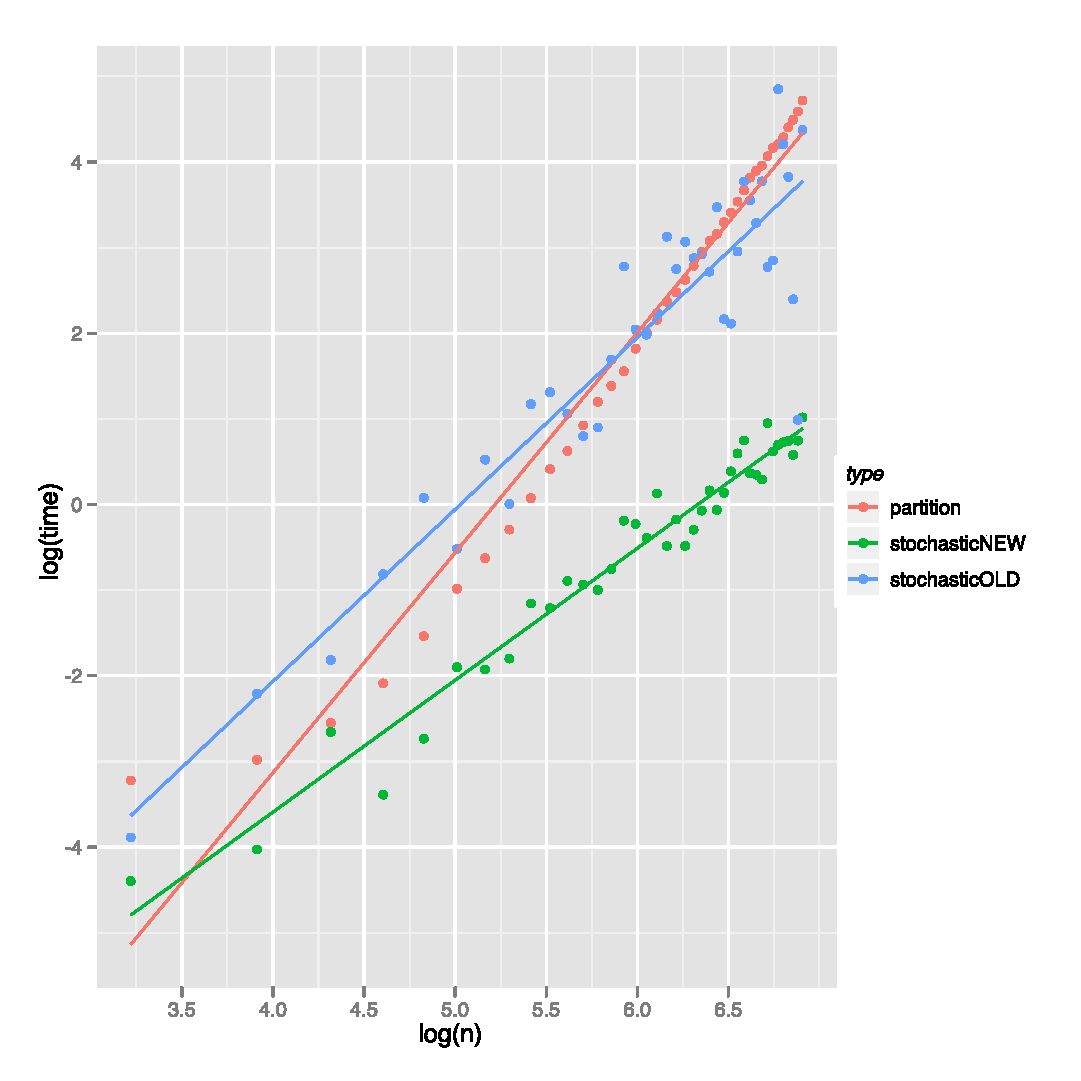
\includegraphics[width=\textwidth]{stochloglog.eps}
\caption[Stochastic Traceback Speedups Log-Log Plot]{Log-Log plots of the timings in Figure
  \ref{fig:stochOvN}. The new stochastic algorithm slope is slightly
  higher than 1, but not much. }
\label{fig:stochLogLog}
\end{figure}
A good question to ask would be, how do we know that this new
algorithm is outputting structures with the correct
probabilities. Verification plot Figure \ref{fig:stochV} attempts to answer that
question.
\begin{figure}
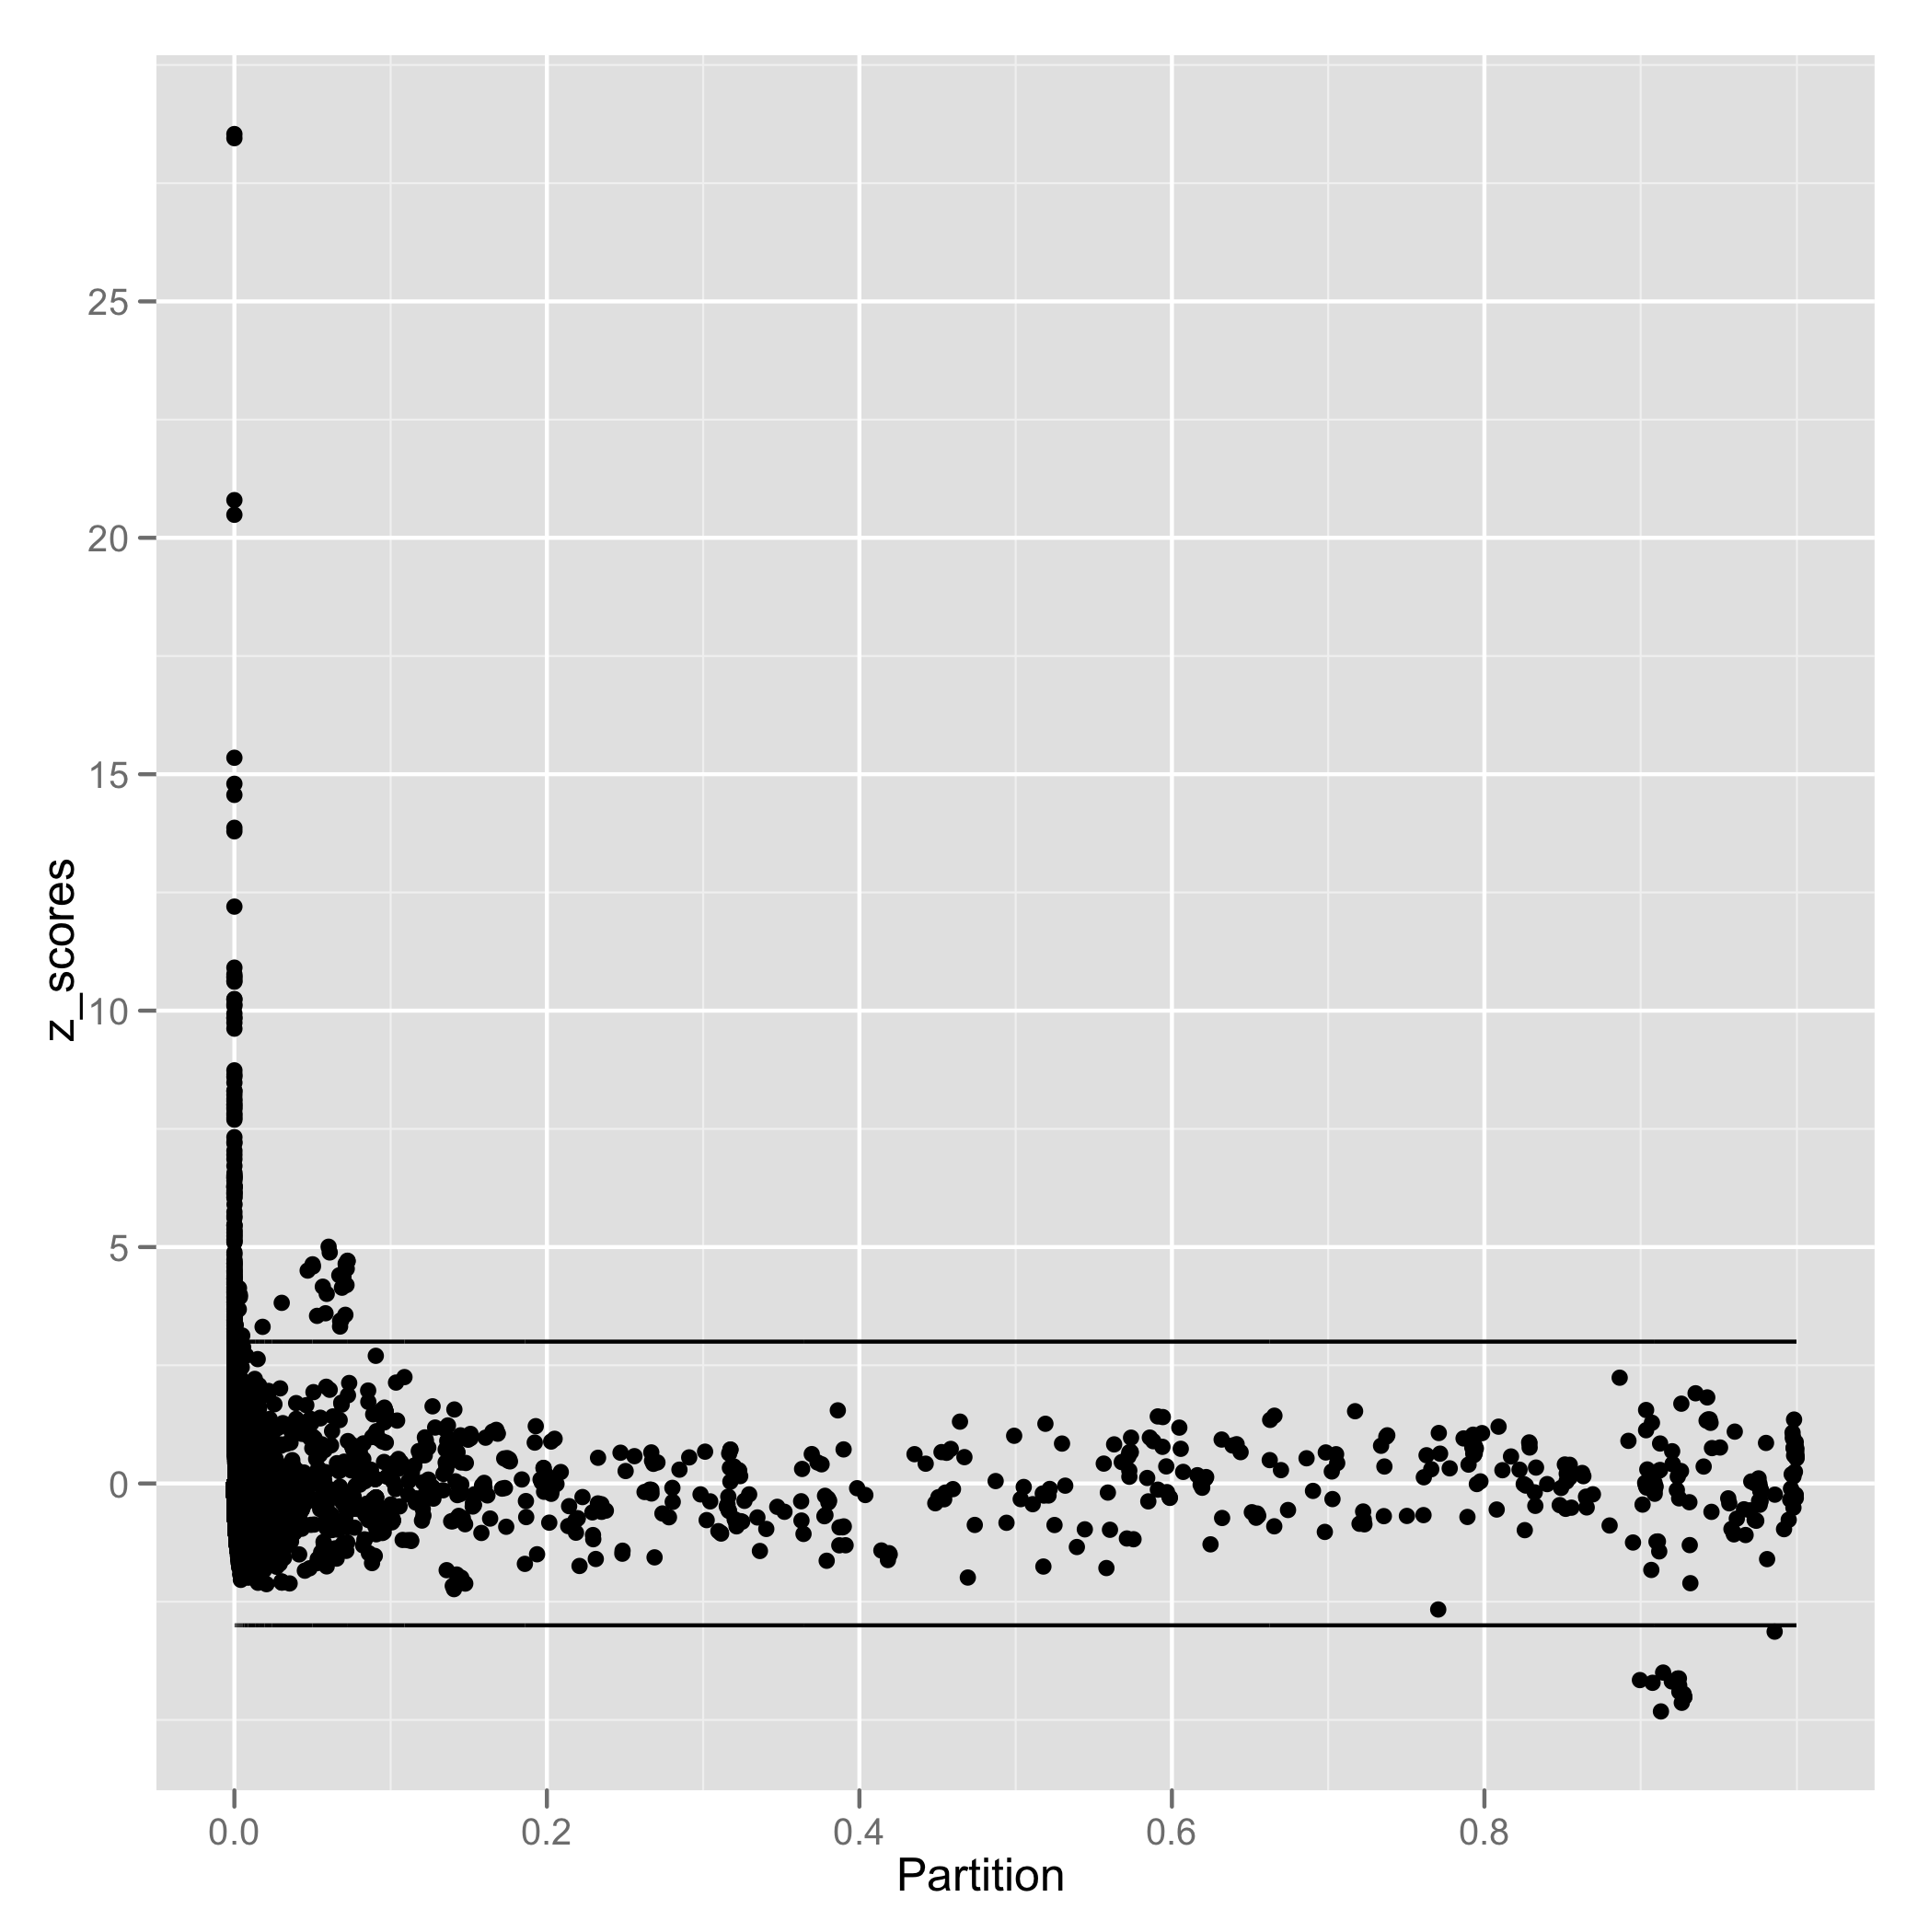
\includegraphics[width=\textwidth]{newzscores.png}
\caption[Stochastic Traceback Verification]{A plot of the difference
  between the partition function probability and the stochastic
  traceback probability of a base pair according to the new
  algorithm. According to the number of states, there should be 30
  states above 0 probability that cross the horizontal lines, there
  are less than 30.}
\label{fig:stochV}
\end{figure}

What we would expect to see from these plots, is that for a given
base, we would expect to see it pair with other bases with
probabilities given by the partition function as one can see. Of
course there is sampling error, so each bin represents a sampling from
a Bernoulli distribution. The number of samples that violate the
bounds do not deviate much from what we would expect from doing $n^2$
experiments, so I think we can confidently say that the new algorithm
is making the correct computation.

%[TODO: Add demonstration of full RAM sampling]

\section{Conclusion}

The stochastic traceback algorithm can be sped up to allow large
amounts of sampling such that the limiting computation factor is
memory, not time. The applications of this improvement are that
statistical algorithms like Ding \& Lawrence \cite{ding2004sfold}
\cite{ding2005rna} can minimize their statistical error. Nestor
\cite{aalbertsNestor} benefits greatly from these improvements because
more structures mean more branches to the tree. In general the
algorithm is useful because it removes unnecessary computation that
was done before.

%% This is an example first chapter.  You should put chapter/appendix that you
%% write into a separate file, and add a line \include{yourfilename} to
%% main.tex, where `yourfilename.tex' is the name of the chapter/appendix file.
%% You can process specific files by typing their names in at the 
%% \files=
%% prompt when you run the file main.tex through LaTeX.
\chapter{Nestor and Clustering}
\section{Motivation}

Given that we know, for any given RNA strand, the probability of an
individual state is very low [TODO: reference section], a much more
important computation is the overall shape of the strand's free energy
landscape. Even if the probability of an individual state is low, if
we "integrate" over a basin of free energy, the probability of that
set of states could be something tangible.

In the past 10 years, several groups have started to explore this
concept. There are two approaches, in general, to define basins and
classify structures into them. The first class of methods defines the
basins from the top-down: given a number of stochastically sampled
structures, we divide them into groups based on some kind of distance
metric. These methods tend to be very similar to typical clustering
algorithms used in computer science and data analysis.

Another approach is to start at local minima and climb up the energy
barriers between minima using the metropolis-hastings algorithm to
maintain the correct probabilities according to the partition
function. These methods can be used to accurately compute the energies
of the transition states between local minima and these can tell you
the kinetics of the structure. This technique was developed by [TODO:
find Vienna people and cite them].

\section{Nestor}

Enabled by the stochastic traceback algorithm to sample large numbers
of states from the Boltzmann distribution, the Nestor algorithm,
developed by Aalberts and Jannen, uses a different measure of
distance based on the number of conflicting pairs between two
structures. This measure is called nestedness and it is defined as
$\Psi^{\mu\nu}$ between structures $\mu$ and $\nu$, such that

\begin{equation}
\Psi^{\mu\nu} = \sum_{k,l} \sum_{m,n \times (k,l)} P^{\mu}_{kl}
P^{\nu}_{mn} 
\end{equation}

The algorithm works as follows: given an ensemble of structures $S$,
find the most non-nested pair, $p$, from $S$ and sort the structures
into 2 groups: structures compatible (non-crossing) with $p$ and not
compatible (crossing) $p$. These two sub ensembles become the children
of $S$ in a tree that is constructed by recursively splitting
ensembles in the same manner.

%% This is an example first chapter.  You should put chapter/appendix that you
%% write into a separate file, and add a line \include{yourfilename} to
%% main.tex, where `yourfilename.tex' is the name of the chapter/appendix file.
%% You can process specific files by typing their names in at the 
%% \files=
%% prompt when you run the file main.tex through LaTeX.
\chapter{Conclusion}

My hopes for this thesis is that it will be of use to someone
interested in doing RNA structure research in the future. Predicting
RNA structure is a very interesting and difficult problem to solve,
but it also contains a variety of open problems that someone new to
the field can jump in and solve. I was very lucky to have been able to
jump in and take some of the low hanging fruit. In addition, I think
my research has opened up many more opportunities for future
researchers to grab more low hanging fruit.

One of these is combining Nestor and Barriers. Nestor is a great top
down approach that focuses on the highest energy conflict between
states to define the macrostates, and Barriers is a very good bottom
up approach that defines physically accurate and conceptually complete
thermodynamic variables. Combining the two approaches could be
fruitful.

Other improvements involve extending the efficiency improvements to
their natural generalization, which includes the pseudoknot
algorithm. This could be the most revolutionary change, because the
improvements to the standard partition function are less significant
since computers are fast enough to compute the largest strands in
reasonable time anyways. This is not true for pseudoknotted partition
functions, and an efficient algorithm could bring it into the realm of
the feasible. This is what is discussed in the next section. 

\section{Future work: Pseudoknot Algorithm}

The partition function algorithm discussed in this thesis and the
literature in general has a crucial flaw that makes it incomplete. The
algorithm assumes that RNA secondary structure is `well nested', that
there are no overlapping pairs $(i, j)$ and $(k, l)$ such that one of
$k$ or $l$ is between $i$ and $j$ and the other is not.

It is not true that RNA secondary structures are well-nested in
general. When a non-nested pair is present in a secondary structure,
that structure is said to contain a `pseudoknot'. Large groups of
classified RNA sequences such as Group I Introns (around 6\%
pseudeoknotted) and RNase P (around 13\% pseudoknotted) have
pseudoknots in their chemically determined secondary structure, and it
is in these groups that secondary structure prediction performs the
worst (Matthews et all 1999). Large RNA molecules tend to have
pseudoknots, which is unfortunate because the partition function
computation scales much worse when pseudoknots are included.

In general, computation of pseudoknotted structures is hard. In fact,
the problem has been shown to be NP-Complete. Algorithms
to perform the computation for a signficiant subset of pseudoknots
have been designed, most notably by Dirks and Pierce, who have
specified an $O(n^8)$ algorithm and a $O(n^5)$ simplification of that
algorithm, using the same approximations used to reduce the complexity
of the internal loop energy computation.

I believe the heuristic approach of only iterating over allowed pairs
will be able to significantly speed up the pseudoknot
computation. This could be truly revolutionary, because there is no
software that currrently includes pseudoknots in the computation of
the partition function. Since the algorithms seem to perform the worst
in high-pseudoknot structure groups, this could lead to a significant
improvement in RNA structure prediction. 

However, this would require a good energy model for pseudoknots to be
developed. There currently is only one pseudoknot energy model, it is
in the Dirks and Peirce paper \cite{dirks2003partition}. However this
energy model is not physically based, and is just a linear energy
model with a penalty for starting a pseudoknot and a constant bonus
for adding pairs. As we have seen with the standard energy model, this
approach does not capture enough interaction between terms, so a new
energy model needs to be specified. This could be another low hanging
fruit. 

\appendix
\chapter{UNAfold Implementation of Partition Function Improvements}

Note the terms $Z_{ND}$, $Z_{3'D}$, $Z_{5'D}$, and $Z_{DD}$ are extra
free energy terms corresponding to 'dangle energies' which are the
results of an experiment later implemented in the model to improve it
from the standard energy model. In addition there are AU penalty terms
appended to where pairs are made, as AU and GU pairs have penalties
associated with forming. These additional energy terms improve the
model's predictive ability and bring the model closer to the "truth",
however it unfortunately makes the partition function seem very
threatening.


\section{New Q(i,j) derivation}

In UNAfold, we have that the old recurrence relations were as follows:

\begin{equation}
Q(i,j) = \sum_{k=i}^j \left ( Q(i, k-1) + e^{-\frac{b(k-i)}{RT}}  \right )Q^1(k, j)
\end{equation}
where 
\begin{equation}
\begin{split}
Q^1(i, j) = \ \ & Q^1(i, j - 1) e^{-\frac{b}{RT}}  \\
 +\ & e^{-\frac{c}{RT} }Z_{ND}(i, j) Q'(i, j)  \\
+\ & e^{-\frac{b + c}{RT}}Z_{5'D}(i + 1, j)Q'(i + 1, j)  \\
+\ &  e^{-\frac{b + c}{RT}}Z_{3'D}(i, j-1)Q'(i, j - 1)  \\
+\ &  e^{-\frac{2b + c}{RT}}Z_{DD}(i + 1, j-1)Q'(i + 1, j-1) 
\end{split}
\end{equation}
\noindent
We can expand the recursive definition of $Q^1(i,j)$:

\begin{equation}
\begin{split}
Q^1(i, j) = \sum_{k' = i + 1}^j e^{-\frac{b(j - k')}{RT} } \bigg [ \ 
  & e^{-\frac{c}{RT} }Z_{ND}(i, k') Q'(i, k') \\
 +\ & e^{-\frac{b + c}{RT}}Z_{5'D}(i + 1, k')Q'(i + 1, k') \\ 
+\  & e^{-\frac{b + c}{RT}}Z_{3'D}(i, k'-1)Q'(i, k' - 1) \\
+\  & e^{-\frac{2b + c}{RT}}Z_{DD}(i + 1, k'-1)Q'(i + 1, k'-1) \   \bigg ]
\end{split}
\end{equation}
\noindent
Plugging this into $Q(i,j)$ we get:

\begin{equation}
\begin{split}
Q(i, j) = \sum_{k= i}^j\ \sum_{k' = k + 1}^j \left (  Q(i, k-1) + e^{-\frac{b(k-i)}{RT}} \right ) e^{-\frac{b(j - k')}{RT} } \bigg [ \ 
  & e^{-\frac{c}{RT} }Z_{ND}(k, k') Q'(k, k')  \\
+\  & e^{-\frac{b + c}{RT}}Z_{5'D}(k + 1, k')Q'(k + 1, k') \\ 
+\ & e^{-\frac{b + c}{RT}}Z_{3'D}(k, k'-1)Q'(k, k' - 1) \\
+\  & e^{-\frac{2b + c}{RT}}Z_{DD}(k + 1, k'-1)Q'(k + 1, k'-1) \   \bigg ]
\end{split}
\end{equation}
\noindent
Now we'll take the $j$th element of the second sum and split it out (note that the $j$th part of the 1st sum has no elements to sum now, so we can decrement that too):
\begin{equation}
\begin{split}
Q(i, j) = \sum_{k= i}^{j-1}\ \sum_{k' = k + 1}^{j-1} \left (  Q(i, k-1) + e^{-\frac{b(k-i)}{RT}} \right ) e^{-\frac{b(j - k')}{RT} } \bigg [ \ 
  & e^{-\frac{c}{RT} }Z_{ND}(k, k') Q'(k, k')  \\
+ \  & e^{-\frac{b + c}{RT}}Z_{5'D}(k + 1, k')Q'(k + 1, k')\\ 
+\   & e^{-\frac{b + c}{RT}}Z_{3'D}(k, k'-1)Q'(k, k' - 1) \\
+\  & e^{-\frac{2b + c}{RT}}Z_{DD}(k + 1, k'-1)Q'(k + 1, k'-1) \   \bigg ] \\
+\ \sum_{k=i}^j  \left (  Q(i, k-1) + e^{-\frac{b(k-i)}{RT}} \right ) \bigg [ \ 
  & e^{-\frac{c}{RT} }Z_{ND}(k, j) Q'(k, j) \\
+\  & e^{-\frac{b + c}{RT}}Z_{5'D}(k + 1, j)Q'(k + 1, j) \\ 
+\  & e^{-\frac{b + c}{RT}}Z_{3'D}(k, j-1)Q'(k, j - 1) \\
 +\  & e^{-\frac{2b + c}{RT}}Z_{DD}(k + 1, j-1)Q'(k + 1, j-1) \   \bigg ]
\end{split}
\end{equation}
\noindent
Notice that the double sum is simply $Q(i,j-1)e^{-b/RT}$ and the terms of the second, single sum are over the pairs with $j$ or $j-1$. Therefore, we can use our heuristic for the pairs of $j$ and $j-1$ to produce the following computation for $Q(i, j)$ which is much more efficient than the previous ones:
\begin{equation}
\begin{split}
Q(i,j) = Q(i, j-1)e^{-b/RT} +  \sum_{k(j)} & \bigg [  \left (  Q(i, k-1) + e^{-\frac{b(k-i)}{RT}} \right ) \
   e^{-\frac{c}{RT} }Z_{ND}(k, j) Q'(k, j)  \\
+\ & \left (  Q(i, k-2) + e^{-\frac{b(k-i-1)}{RT}} \right )    e^{-\frac{b + c}{RT}}Z_{5'D}(k, j)Q'(k, j) \   \bigg ]  \\
+\  \sum_{l(j-1)} & \bigg [  \left (  Q(i, l-1) + e^{-\frac{b(l-i)}{RT}} \right ) \
   e^{-\frac{c}{RT} }Z_{ND}(l, j-1) Q'(l, j-1)  \\
+\ & \left (  Q(i, l-2) + e^{-\frac{b(l-i-1)}{RT}} \right )   e^{-\frac{2b + c}{RT}}Z_{DD}(l, j-1)Q'(l, j-1) \   \bigg ] 
\end{split}
\end{equation}

\section{Derivation of new Q'(i, j) formula}
For $Q'(i, j)$ we start with the recursion:

\begin{equation}
\begin{split}
Q'(i,j) = Z_H(i, j) &+ Z_S(i, j) Q'(i+1, j-1) + QBI(i, j) \\
+\ & e^{-\frac{a+c}{RT}}Z_{ND}(j, i) \sum_{k = i + 3}^{j-5}Q(i+1, k - 1)Q^1(k, j-1)  \\
+\ & e^{-\frac{a+b+c}{RT}}Z_{3'D}(j, i) \sum_{k = i + 4}^{j-5}Q(i+2, k - 1)Q^1(k, j-1)  \\
+\ & e^{-\frac{a+b+c}{RT}}Z_{5'D}(j, i) \sum_{k = i + 3}^{j-6}Q(i+1, k - 1)Q^1(k, j-2) \\
+\ & e^{-\frac{a+2b+c}{RT}}Z_{DD}(j, i) \sum_{k = i + 4}^{j-6}Q(i+2, k - 1)Q^1(k, j-2) 
\end{split}
\end{equation}
\noindent
The 4 for loops in this make this an expensive computation as the number of bases gets very high. However, these for loops are very similar to the partition function in structure. Indeed, we could perhaps replace each of them with a function of the form $Q^m(i, j)$ defined as

\begin{equation}
Q^m(i, j) = \sum_{k = i +3}^{j-5} Q(i + 1, k - 1) Q^1(k, j - 1)
\end{equation} 
\noindent
Which would simplify the previous sum to a constant time computation, provided we have memoized $Q^m$:
\begin{equation}
\begin{split}
Q'(i,j) = Z_H(i, j) &+ Z_S(i, j) Q'(i+1, j-1) + QBI(i, j)  \\
+\ & e^{-\frac{a+c}{RT}}Z_{ND}(j, i) Q^m(i, j)  \\
+\ & e^{-\frac{a+b+c}{RT}}Z_{3'D}(j, i) Q^m( i + 1, j) \\
+\ & e^{-\frac{a+b+c}{RT}}Z_{5'D}(j, i) Q^m(i, j- 1) \\
+\ & e^{-\frac{a+2b+c}{RT}}Z_{DD}(j, i) Q^m(i + 1, j -1)
\end{split}
\end{equation}

\noindent
Now there just needs to be a way to efficiently compute $Q^m$. First we substitute in the expanded version of $Q^1$:

\begin{equation}
\begin{split}
Q^m(i, j) = \sum_{k = i + 3}^{j - 5}\  \sum_{k' = k + 1}^{j- 1} Q(i + 1, k - 1)  e^{-\frac{b(j - k')}{RT} } \bigg [ \ 
  & e^{-\frac{c}{RT} }Z_{ND}(k, k') Q'(k, k') \\
+\  & e^{-\frac{b + c}{RT}}Z_{5'D}(k + 1, k')Q'(k + 1, k') \\ 
 +\ & e^{-\frac{b + c}{RT}}Z_{3'D}(k, k'-1)Q'(k, k' - 1) \\
+\  & e^{-\frac{2b + c}{RT}}Z_{DD}(k + 1, k'-1)Q'(k + 1, k'-1) \   \bigg ]
\end{split}
\end{equation}

\noindent
Then we do as before and seperate out the $j$th term of the second sum. Note that there seems to be an additional sum needed to account that I've decreased the first sum's endpoint to $j-6$, but the sum ends up being from $k'= j-4$ to $k' = j -2$ and since $Q'$ for bases less than 4 apart is 0 due to hairpin loop rules, this sum is equal to zero.
\begin{equation}
\begin{split}
Q^m(i, j) = \sum_{k = i + 3}^{j - 6}\  \sum_{k' = k + 1}^{j- 2} Q(i + 1, k - 1)  e^{-\frac{b(j - k'-1)}{RT} } \bigg [ \ 
  & e^{-\frac{c}{RT} }Z_{ND}(k, k') Q'(k, k') \\
+ \  & e^{-\frac{b + c}{RT}}Z_{5'D}(k + 1, k')Q'(k + 1, k') \\ 
+ \  & e^{-\frac{b + c}{RT}}Z_{3'D}(k, k'-1)Q'(k, k' - 1) \\
 + \  & e^{-\frac{2b + c}{RT}}Z_{DD}(k + 1, k'-1)Q'(k + 1, k'-1) \   \bigg ]\\
+ \ \sum_{k = i + 3}^{j - 5}\ Q(i + 1, k - 1)  \bigg [ \ 
  & e^{-\frac{c}{RT} }Z_{ND}(k, j-1) Q'(k, j-1)  \\
+ \  & e^{-\frac{b + c}{RT}}Z_{5'D}(k + 1, j-1)Q'(k + 1, j-1) \\ 
  + \ & e^{-\frac{b + c}{RT}}Z_{3'D}(k, j-2)Q'(k, j-2)\\
+ \  & e^{-\frac{2b + c}{RT}}Z_{DD}(k + 1, j-2)Q'(k + 1, j-2) \   \bigg ]\ 
\end{split}
\end{equation}
\noindent
The double sum is again going to be equal to $Q^m(i, j -1)e^{-b/RT}$, and the second sum can be made much more efficient by our heuristic. 
\begin{equation}
\begin{split}
Q^m(i, j) = Q^m(i, j - 1)e^{-b/RT} + \sum_{k(j - 1)} \bigg [ & Q(i + 1, k - 1)   
  e^{-\frac{c}{RT} }Z_{ND}(k, j-1) Q'(k, j-1)  \\
 + \ &Q(i + 1, k - 2) e^{-\frac{b + c}{RT}}Z_{5'D}(k, j-1)Q'(k, j-1)  \bigg ]\ \\
+ \sum_{k(j-2)} \bigg [ & Q(i + 1, k - 1)   
  e^{-\frac{c}{RT} }Z_{3'D}(k, j-2) Q'(k, j-2)  \\
  +\ &Q(i + 1, k - 2) e^{-\frac{b + c}{RT}}Z_{DD}(k, j-2)Q'(k, j-2)  \bigg ]
\end{split}
\end{equation}
\noindent

Since the $k$s for any individual $j$ are found to be quite limited, the final form should be much more efficient at computing the $Q'(i, j)$.

Note that for $Q$ and in many places for $Q'$, instead of a sum over
the known $k$ that could possibly begin a leftmost pair, we see a
double sum. One of them over $k$ that could end a leftmost pair, and
this sum is limited to a certain length below $j$. This is just making
the same assumption that the internal loop computation makes: there
are not arbitrarily long strands without base pairs, after a certain
number of bases it becomes overwhelmingly more likely to make a base
pair that we can virtually ignore the energy of the the cases of
length beyond a certain $L$.

As for the seocnd sum, since the number of probable pairs for a base
$i$ has been shown empirically to be roughly constant, regardless of
length, the second sum is essentially constant. What this all means is
that all $O(n^2)$ computations of $Q(i,j)$'s are roughly constant
time. This means that the overall algorithm is $O(n^2)$, an
improvement over the previous algorithms asymptotic bound by and order
of $n$.


%% This defines the bibliography file (main.bib) and the bibliography style.
%% If you want to create a bibliography file by hand, change the contents of
%% this file to a `thebibliography' environment.  For more information 
%% see section 4.3 of the LaTeX manual.
\begin{singlespace}
\bibliography{main}
\bibliographystyle{plain}
\end{singlespace}

\end{document}

